\section{问题二：异构无人机多点多架次运输调度}

\subsection{模型建立}

问题二将问题一的单点往返扩展为多点多架次调度：每个运输架次可访问一个或多个服务区（O01$\to$Si$\to$Sj$\to\cdots\to$O01），需在实体机队、共享电池与硬时限约束下联合确定货箱组批、服务区访问顺序、运输机型、执行无人机、共享电池及各架次开始时刻。本节沿用问题一的能耗/时间引擎，新增多站路线、资源调度与多目标三部分。

\subsubsection{多站路线能耗与时间}

对路线 $r$（有序停靠序列 $s_1,\dots,s_k$，起止于 O01），逐腿按当前剩余载荷精确累加能耗（因 $L_g(q)$ 凹、$E^{\rm hor}(q)$ 凸，总能耗与卸货顺序相关，须逐腿计算而非查单点 $q_{\max}$ 表）：
\begin{equation}
E_r = \sum_{(a,b)\in r}\Big[E^{\rm hor}(d_{ab}, q_{ab}) + E^{\rm up}(h^{+}_{ab}, q_{ab})\Big],
\end{equation}
其中 $q_{ab}$ 为进入腿 $a\to b$ 时的剩余载荷。路线可行须满足 $E_r\le(1-\rho)E^{\rm use}_g$、总质量 $\le Q_g$、总体积 $\le V_g$。路线时间 $T_r$ 按起飞一次性准备 + 逐腿飞行 + 逐停靠点交接累加，与问题一 $T^{\rm batch}$ 同口径。

对给定服务区集合的停靠顺序，本文对可行排列精确比较取能耗最低者（非最近邻近似，已自检验证能耗确与顺序相关），并对跨机型选能耗最低的可行机型。

\subsubsection{两阶段充电模型}

共享电池与能源组件作为独立能源资源记录 SOC。从任务结束时 SOC $s$ 充至 100\% 的等效时间按题设两阶段模型\cite{ref_ti}：
\begin{equation}
t^{\rm chg}(s)=
\begin{cases}
T_{\rm full}\left[0.65\dfrac{0.90-s}{0.90}+0.35\right], & 0\le s<0.90,\\[6pt]
T_{\rm full}\cdot 0.35\dfrac{1-s}{0.10}, & 0.90\le s\le 1,
\end{cases}
\end{equation}
其中 $T_{\rm full}$ 为该资源的等效完全充电时间。同一资源的任务占用与充电时段不得重叠，不同资源可并行充电。图~\ref{fig:q2_charge} 给出两阶段充电曲线，可见 90\% 为快充/慢充分界点，快充段占完全充电时间的 65\%。

\begin{figure}[htbp]
\centering
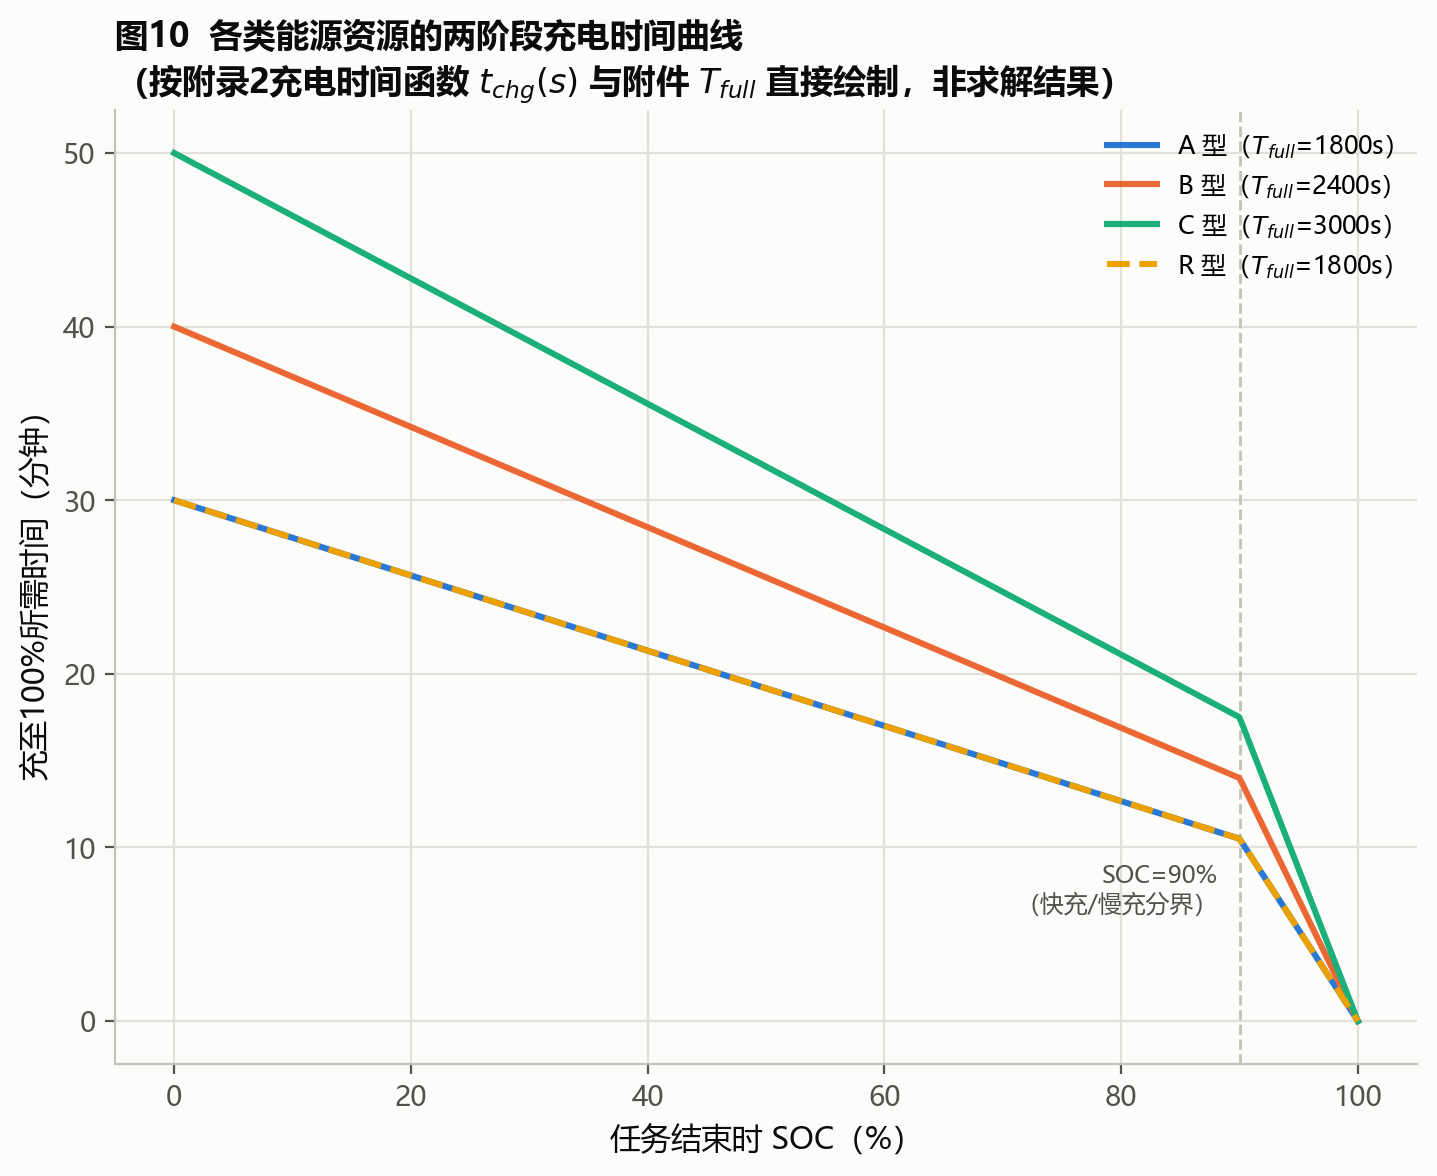
\includegraphics[width=0.6\textwidth]{figures/10_两阶段充电曲线.png}
\caption{两阶段等效充电曲线}
\label{fig:q2_charge}
\end{figure}

\subsubsection{四目标与硬约束分离}

优化目标为四个软目标：配送及时性 $f_1=\sum_i \gamma_i\max(0,t^{\rm arr}_i-t^{\rm exp}_i)$（$\gamma_i$ 为应急优先系数）、全部任务完成时间 $f_2=\max_p t^{\rm end}_p$、运输总能耗 $f_3=\sum_r E_r$、架次数 $f_4$。硬约束（首批截止、医疗期望送达）单独判定为违反量 $V$，不并入 $f_1$，以保持"软目标"与"硬可行性"分离。综合目标记为 $\min\ (f_1,f_2,f_3,f_4)$，且 $V=0$ 优先。

\subsubsection{资源调度约束的离散事件建模}

设架次 $p$ 由机型 $g_p$ 执行，分配无人机 $u_p$ 与电池 $b_p$，起飞时刻 $s_p$、返航时刻 $e_p=s_p+T_{r_p}$（$T_{r_p}$ 为路线飞行与交接时间）。资源可行性由两类不重叠约束刻画：同一架实体无人机的任意两个架次时间区间 $[s_p,e_p]$ 不得重叠；同一组共享电池的任务区间 $[s_p,e_p]$ 与其充电区间 $[e_p,\,e_p+t^{\rm chg}(\mathrm{SOC}_p)]$ 均不得与该电池其他区间重叠。其中架次结束时电池剩余 SOC 由 $\mathrm{SOC}_p=1-E_{r_p}/E^{\rm use}_{g_p}$ 反推，充电时间 $t^{\rm chg}(\cdot)$ 按两阶段充电模型计算。
\begin{equation}
\begin{gathered}
\forall\, p\neq q:\quad \bigl[s_p,e_p\bigr]\cap\bigl[s_q,e_q\bigr]=\varnothing \quad\text{若}\ u_p=u_q\ \text{或}\ b_p=b_q,\\
\forall\, b:\quad \bigl[e_p,\,e_p+t^{\rm chg}(\mathrm{SOC}_p)\bigr]\ \text{与该电池其他任务/充电区间不重叠}.
\end{gathered}
\end{equation}
上述约束经离散事件仿真逐一校验：按起飞时刻排序，为每个架次分配当前空闲的无人机与已充满的电池，逐事件推进时钟，保证所有资源区间不重叠。这一"组批—路线—派单—资源排程"四层耦合结构决定了问题二的难度，也是主方案 NSGA-II 与对比方法贪心构造都必须遵循的公共评价口径。

\subsection{主方案：NSGA-II 全局多目标优化}

主方案采用 NSGA-II 全局分组编码（对应代码 \texttt{q2\_1.py}），以 80 维货箱分组染色体同时编码货箱组批与多站路线：染色体将 80 个货箱划分到若干组，每组按最优停靠顺序与最省能耗机型解码为一条路线，再经离散事件仿真得到 $f_1\sim f_4$ 与违反量 $V$。个体按 Deb 约束支配规则分层排序——先比违反量 $V$（$V=0$ 的可行解优先），可行解间再按 Pareto 支配 + 归一化拥挤度分层\cite{ref_nsga2}。

\begin{algorithm}[htbp]
\caption{问题二主方案：NSGA-II 全局多目标优化（q2\_1.py）}
\LinesNumbered
\KwIn{80 个货箱、15 服务区、3 机型、机队/电池库存、硬时限}
\KwOut{非支配前沿与代表解（架次最少、能耗次优先、$V=0$）}
初始化种群 $P_0$（随机货箱分组编码，规模 80）\;
\For{$t=1$ \KwTo $80$}{
  对每个个体解码为多站路线，经离散事件仿真计算 $(f_1,f_2,f_3,f_4)$ 与违反量 $V$\;
  按 Deb 约束支配规则非支配排序，计算归一化拥挤度\;
  锦标赛选择（先比 $V$，再比非支配层级与拥挤度）\;
  交叉与变异（变异率 0.05，保持分组覆盖 80/80 箱）生成子代 $Q_t$\;
  $P_{t+1}\leftarrow$ 从 $P_t\cup Q_t$ 环境选择前 80 个个体\;
}
返回非支配前沿中 $V=0$、$f_4$ 最小、$f_3$ 次小者作为代表解\;
\end{algorithm}

参数：pilot（种群 24、代数 5）估时后正式种群 80、代数 80。主方案代表解为 $f_1=636937.6$、$f_2=16683.6$\,s（4.63\,h）、$f_3=82.777$\,kWh、$f_4=29$ 架次（多停靠 7 个，占 24.1\%），\textbf{硬约束违反数 $V=0$}，非支配前沿 11 个解全部可行。

图~\ref{fig:q2_nsga} 给出主方案的 Pareto 前沿与路线结构图。由路线结构可见，29 条路线中 22 条为单站直返、7 条为多停靠串访，C 型（仅 2 架机身、4 组电池）承担 10 个架次，是机身排队的瓶颈机队。

\begin{figure}[htbp]
\centering
\subfloat[Pareto 前沿]{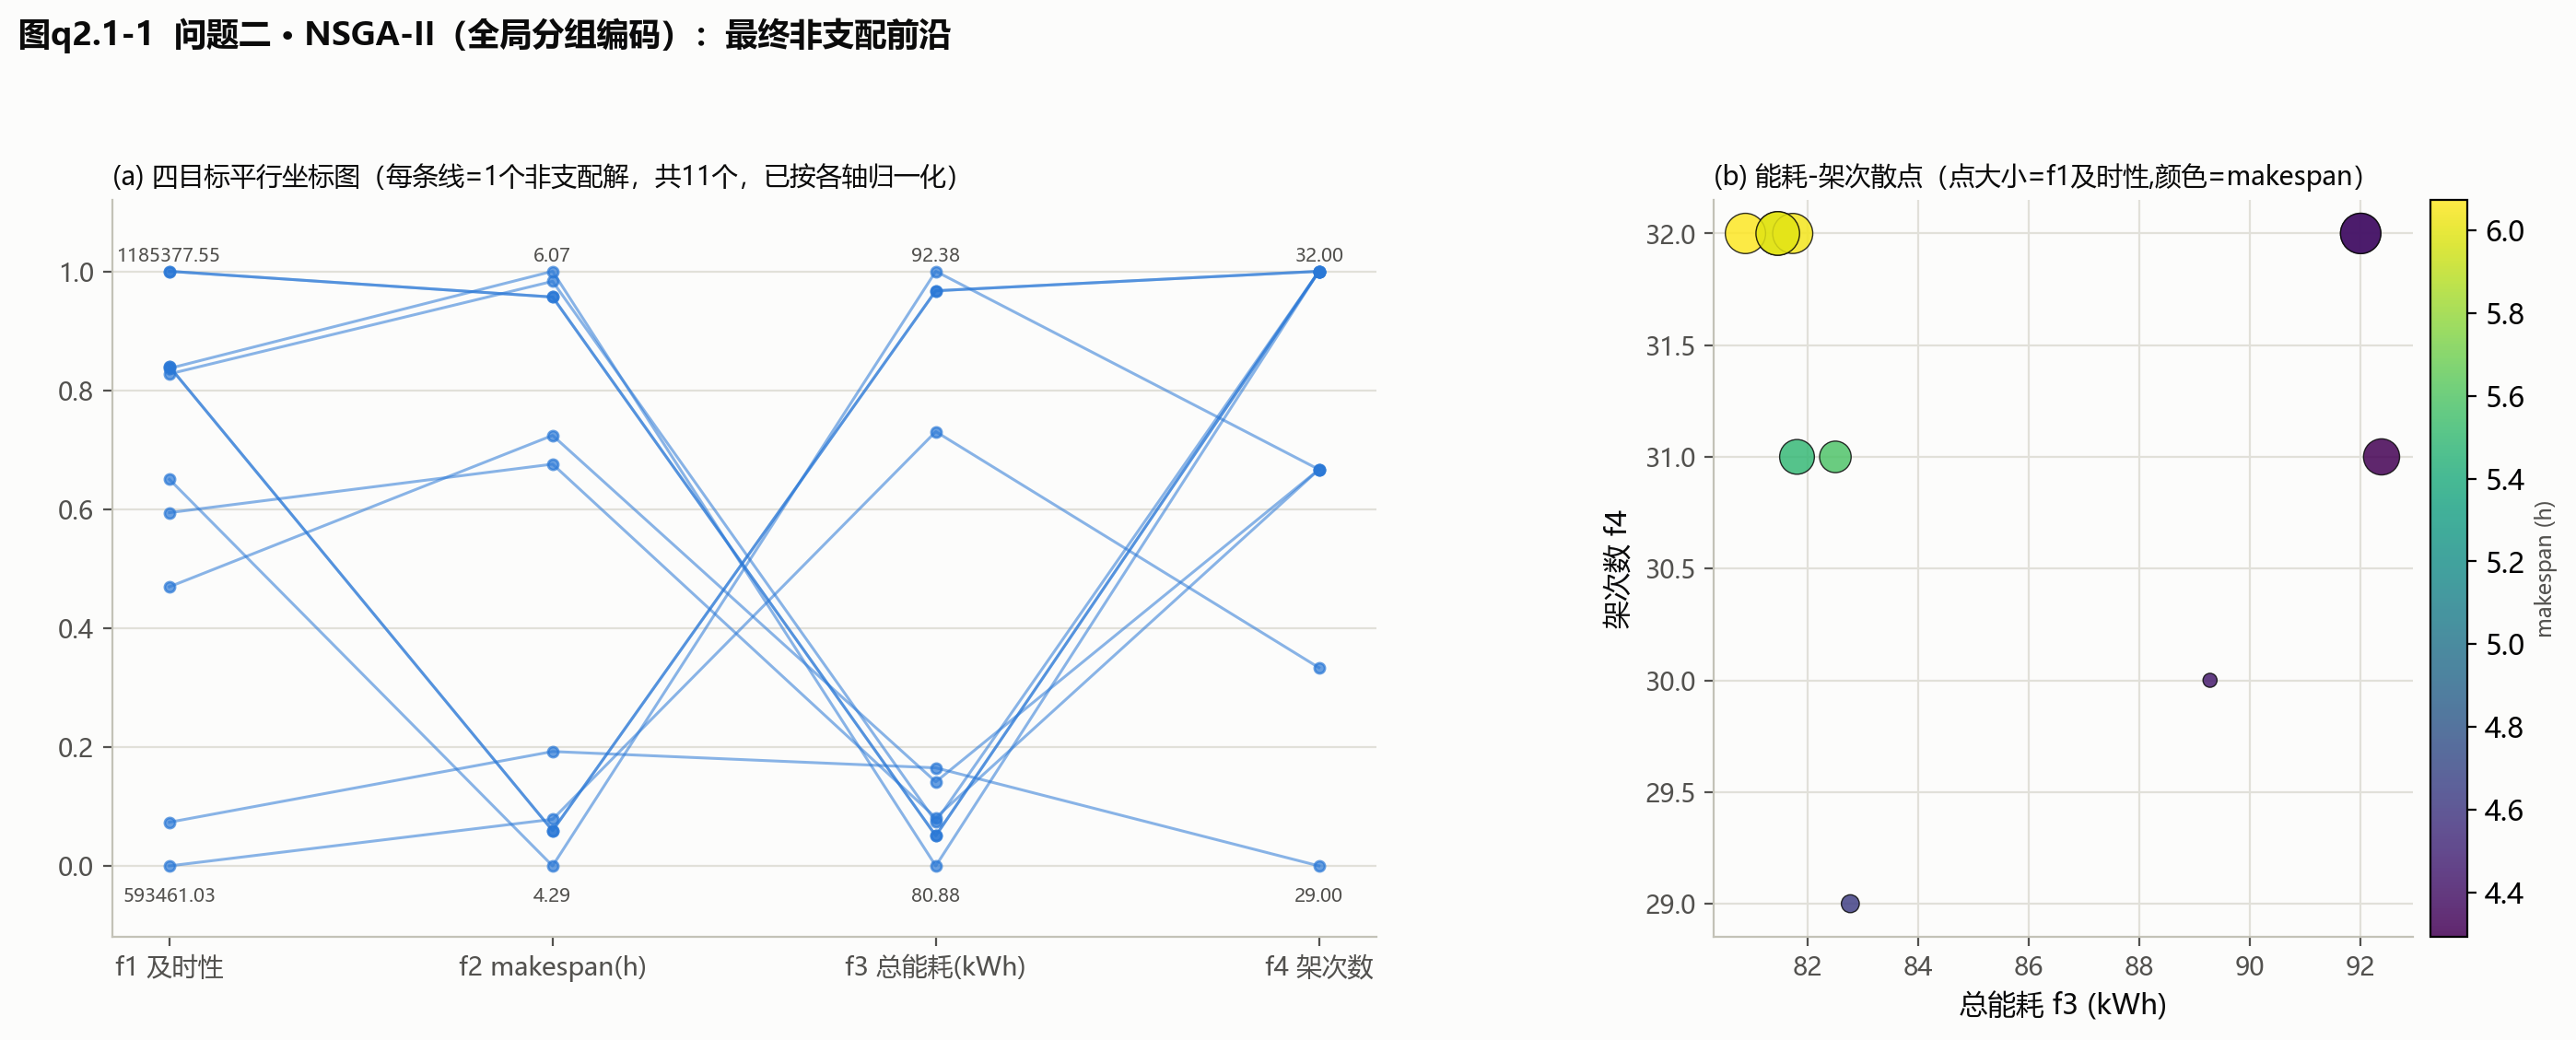
\includegraphics[width=0.48\textwidth]{figures/q2_1_01_帕累托前沿.png}\label{fig:q2_nsga}}
\hfill
\subfloat[NSGA-II 路线结构]{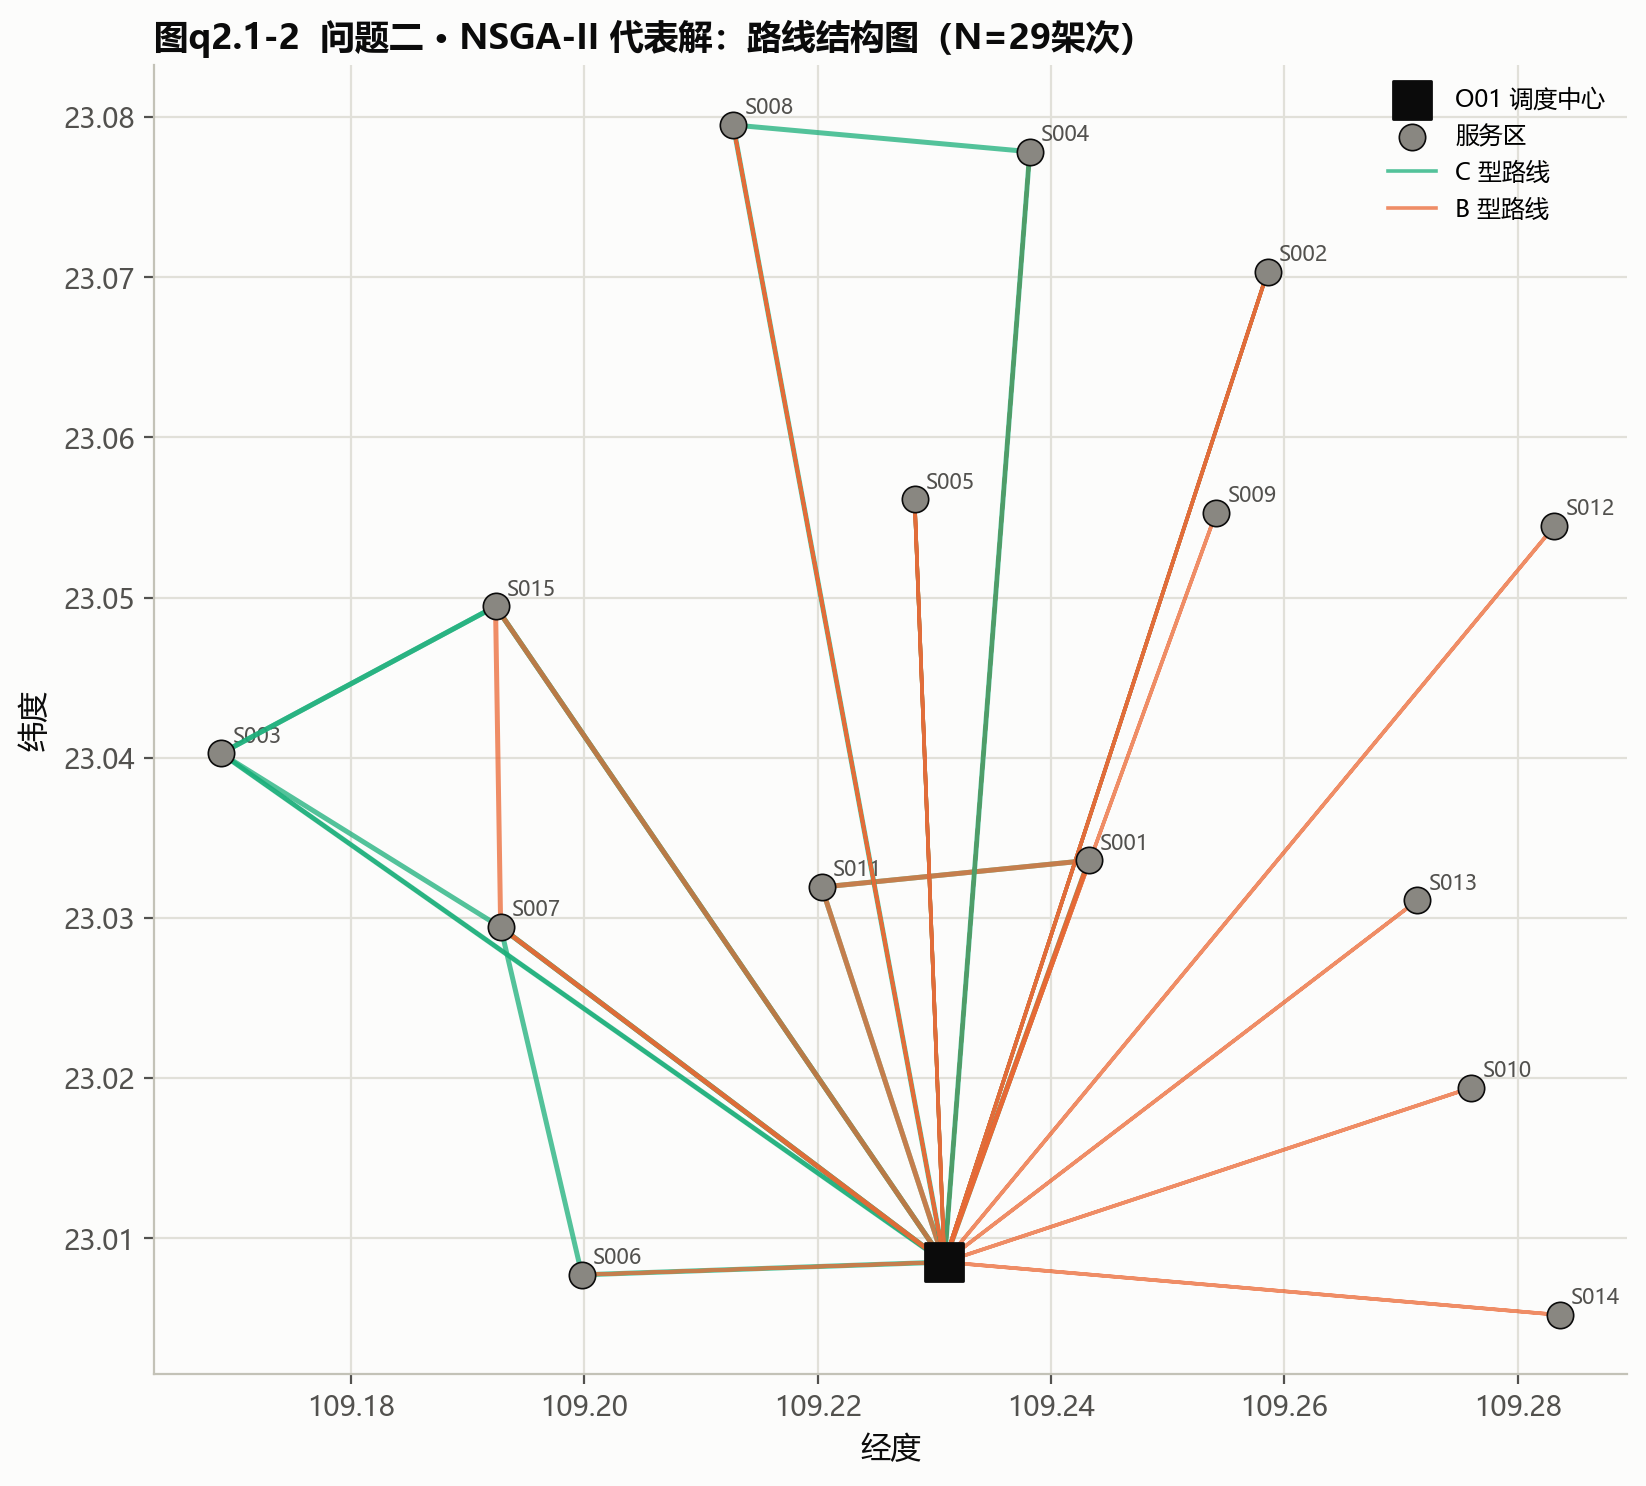
\includegraphics[width=0.48\textwidth]{figures/q2_1_02_路线结构图.png}\label{fig:q2_nsga_route}}
\caption{问题二主方案（NSGA-II）Pareto 前沿与路线结构}
\label{fig:q2_nsga_overview}
\end{figure}

\subsubsection{逐箱送达时刻与配送及时性}

问题要求给出逐箱送达时刻。图~\ref{fig:q2_boxdelivery} 给出 80 个货箱的送达时刻分布：(a) 按服务区分组的逐箱送达散点，(b) 送达时刻的经验累积分布（ECDF）。由于主方案硬约束违反为 0，所有首批保障与医疗物资均在其硬时限内送达，其余货箱的期望送达时间仅作为软目标进入 $f_1$ 度量及时性。

\begin{figure}[htbp]
\centering
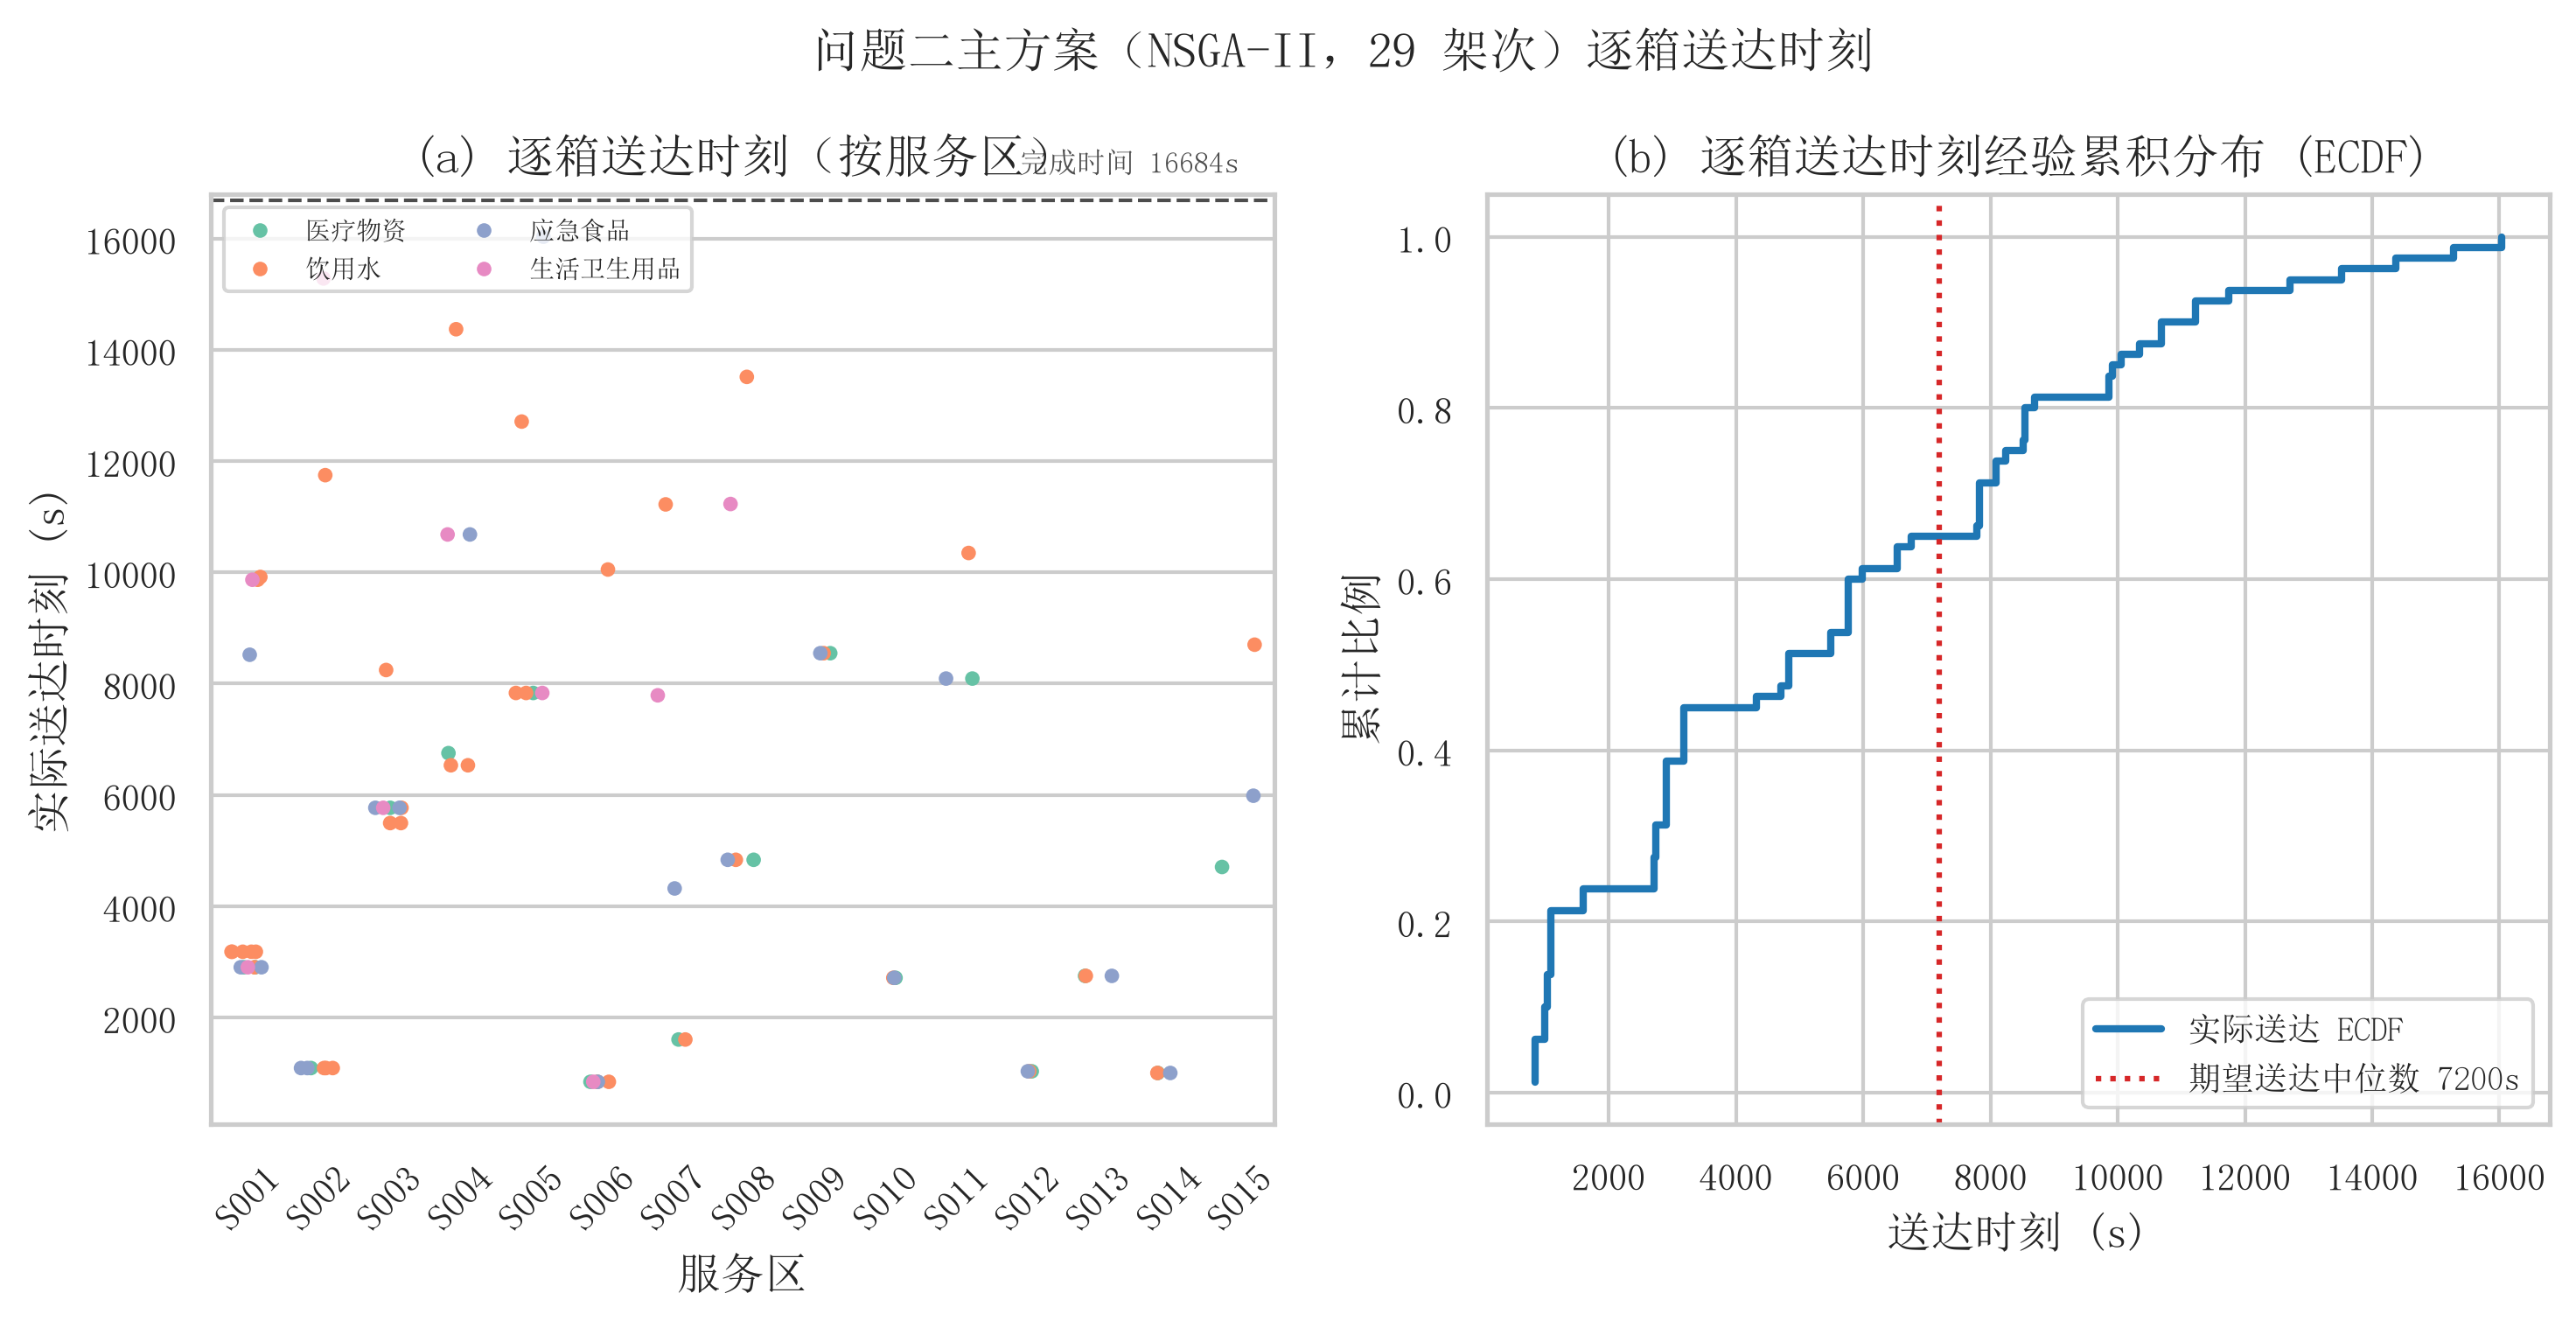
\includegraphics[width=0.95\textwidth]{figures/q2_extra_01_逐箱送达时刻.png}
\caption{问题二主方案逐箱送达时刻分布}
\label{fig:q2_boxdelivery}
\end{figure}

图~\ref{fig:q2_timeliness} 进一步刻画配送及时性：各物资类型的迟到量分布（软目标）与各服务区平均迟到量。可见医疗与首批保障物资因受硬时限约束，迟到量为 0（全部硬时限内送达）；饮用水因数量大、期望时限较宽而存在一定软迟到。图~\ref{fig:q2_svc_heatmap} 给出各服务区各物资类型的平均送达时刻热力图，直观呈现不同服务区的交付节奏差异。

\begin{figure}[htbp]
\centering
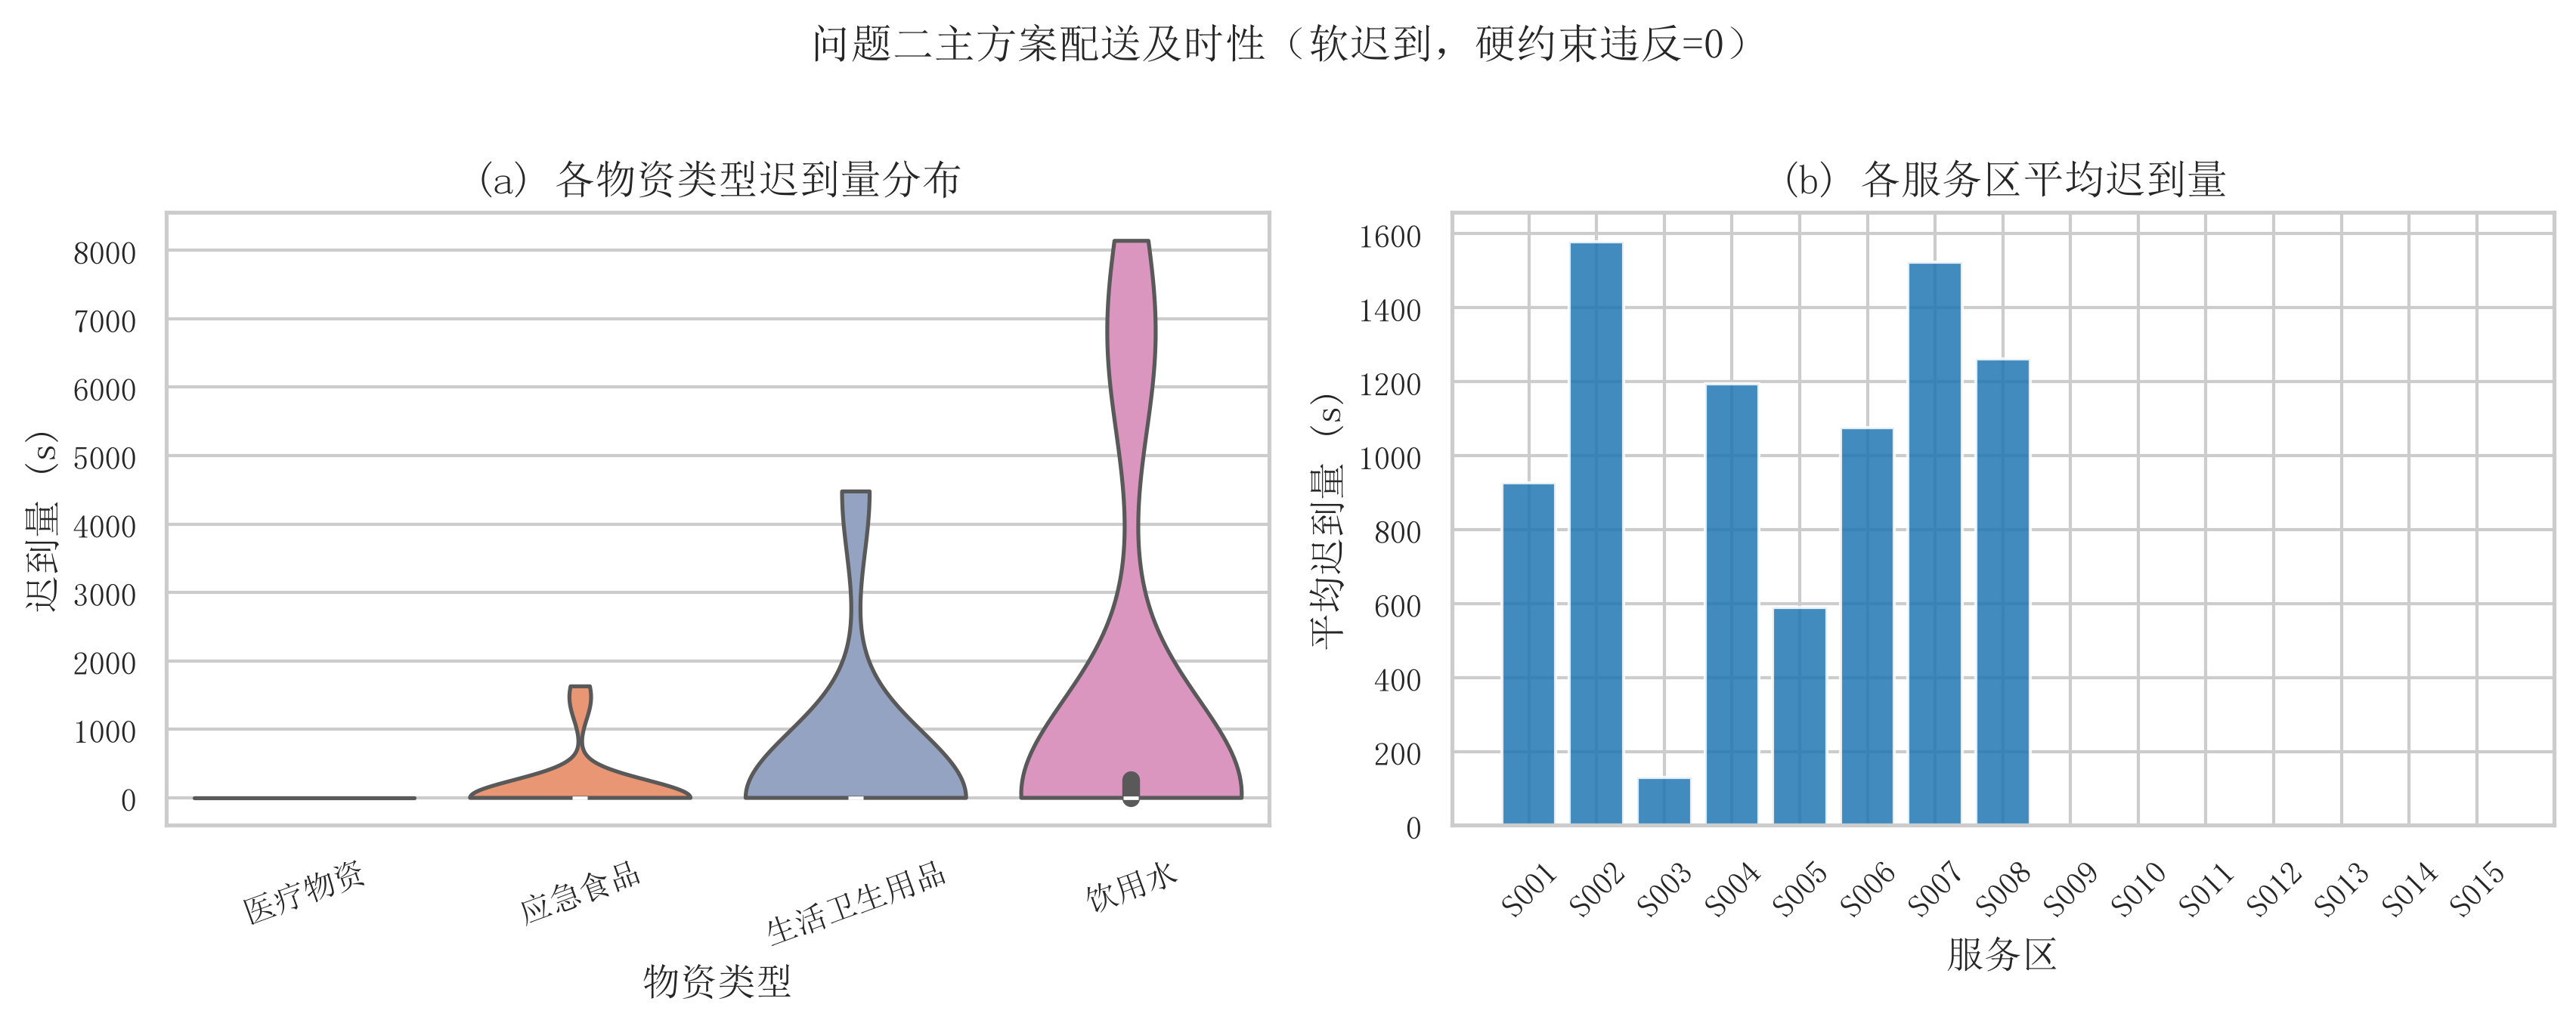
\includegraphics[width=0.95\textwidth]{figures/q2_extra_06_配送及时性分析.png}
\caption{问题二主方案配送及时性分析}
\label{fig:q2_timeliness}
\end{figure}

\begin{figure}[htbp]
\centering
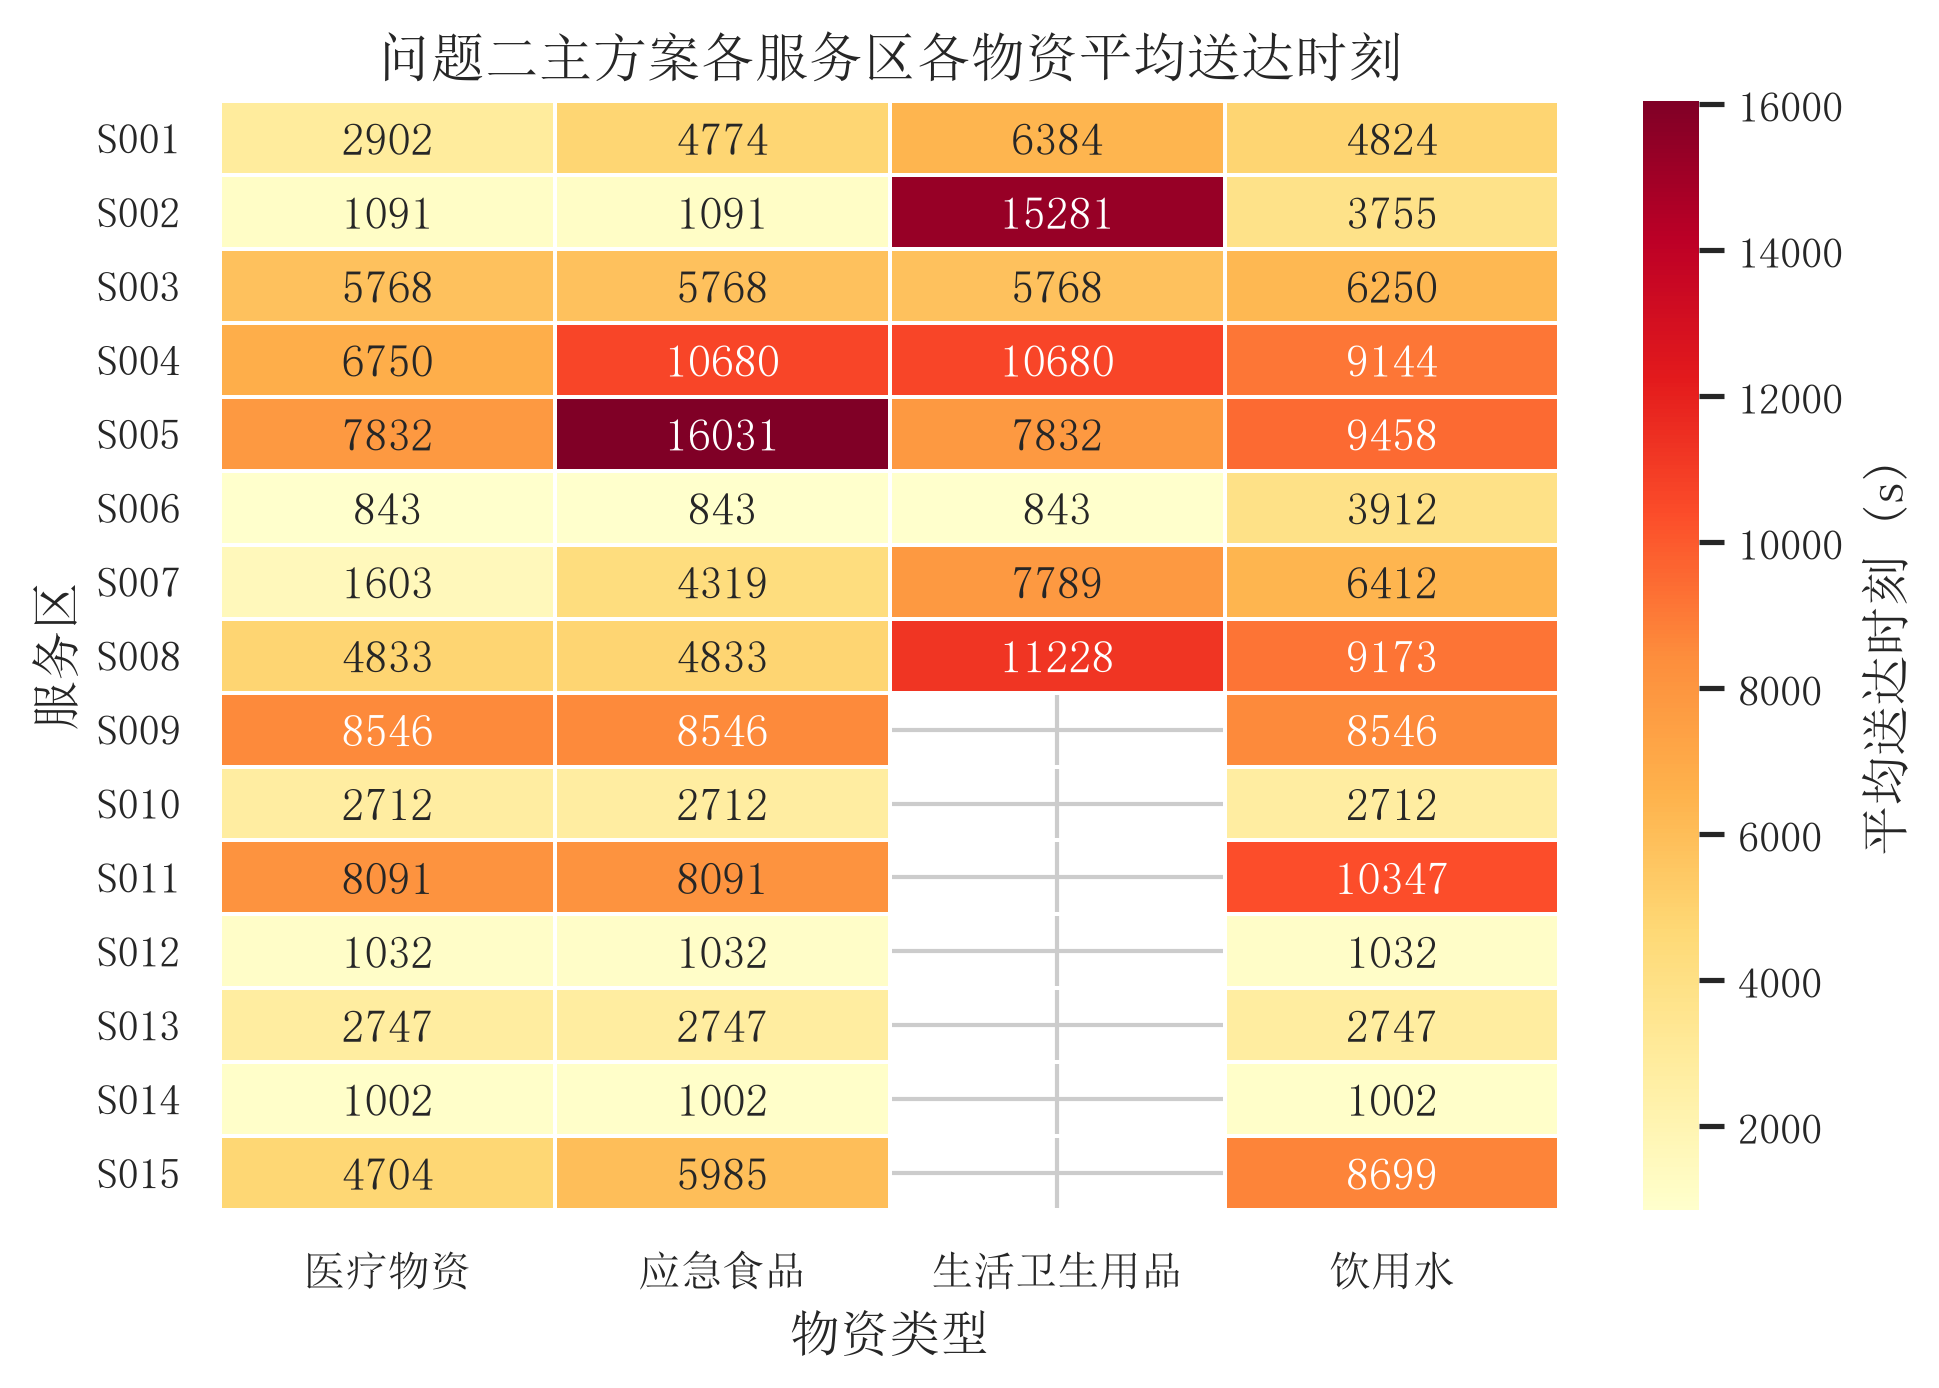
\includegraphics[width=0.75\textwidth]{figures/q2_extra_07_服务区送达时序热力图.png}
\caption{问题二各服务区各物资平均送达时刻}
\label{fig:q2_svc_heatmap}
\end{figure}

图~\ref{fig:q2_conv} 给出 NSGA-II 的收敛过程：种群可行解占比在前 25 代单调上升，第 25 代起全部 80 个个体均成为硬约束可行解，其后进化在四目标前沿上继续优化，印证了"先满足硬可行性、再优化软目标"的搜索路径。

\begin{figure}[htbp]
\centering
\subfloat[可行解占比收敛]{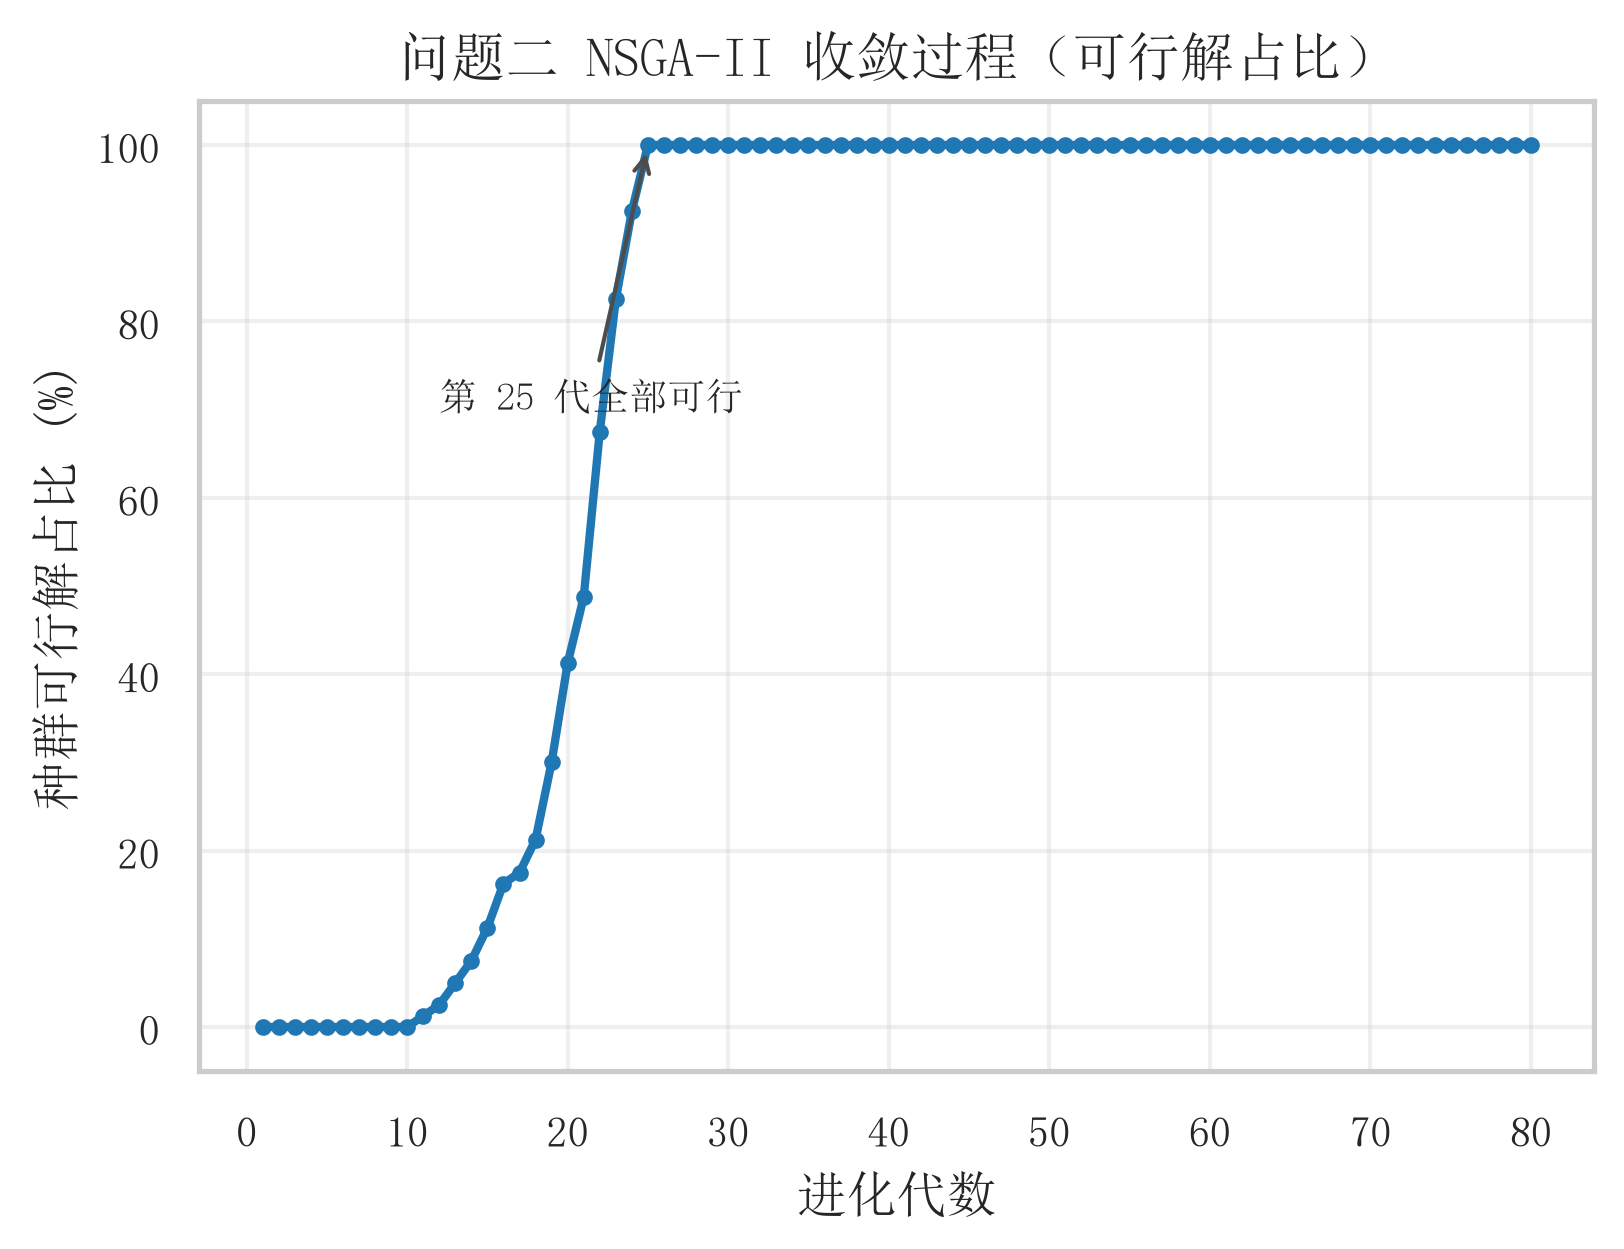
\includegraphics[width=0.48\textwidth]{figures/q2_extra_02_NSGA2收敛曲线.png}\label{fig:q2_conv}}
\hfill
\subfloat[非支配前沿三维视角]{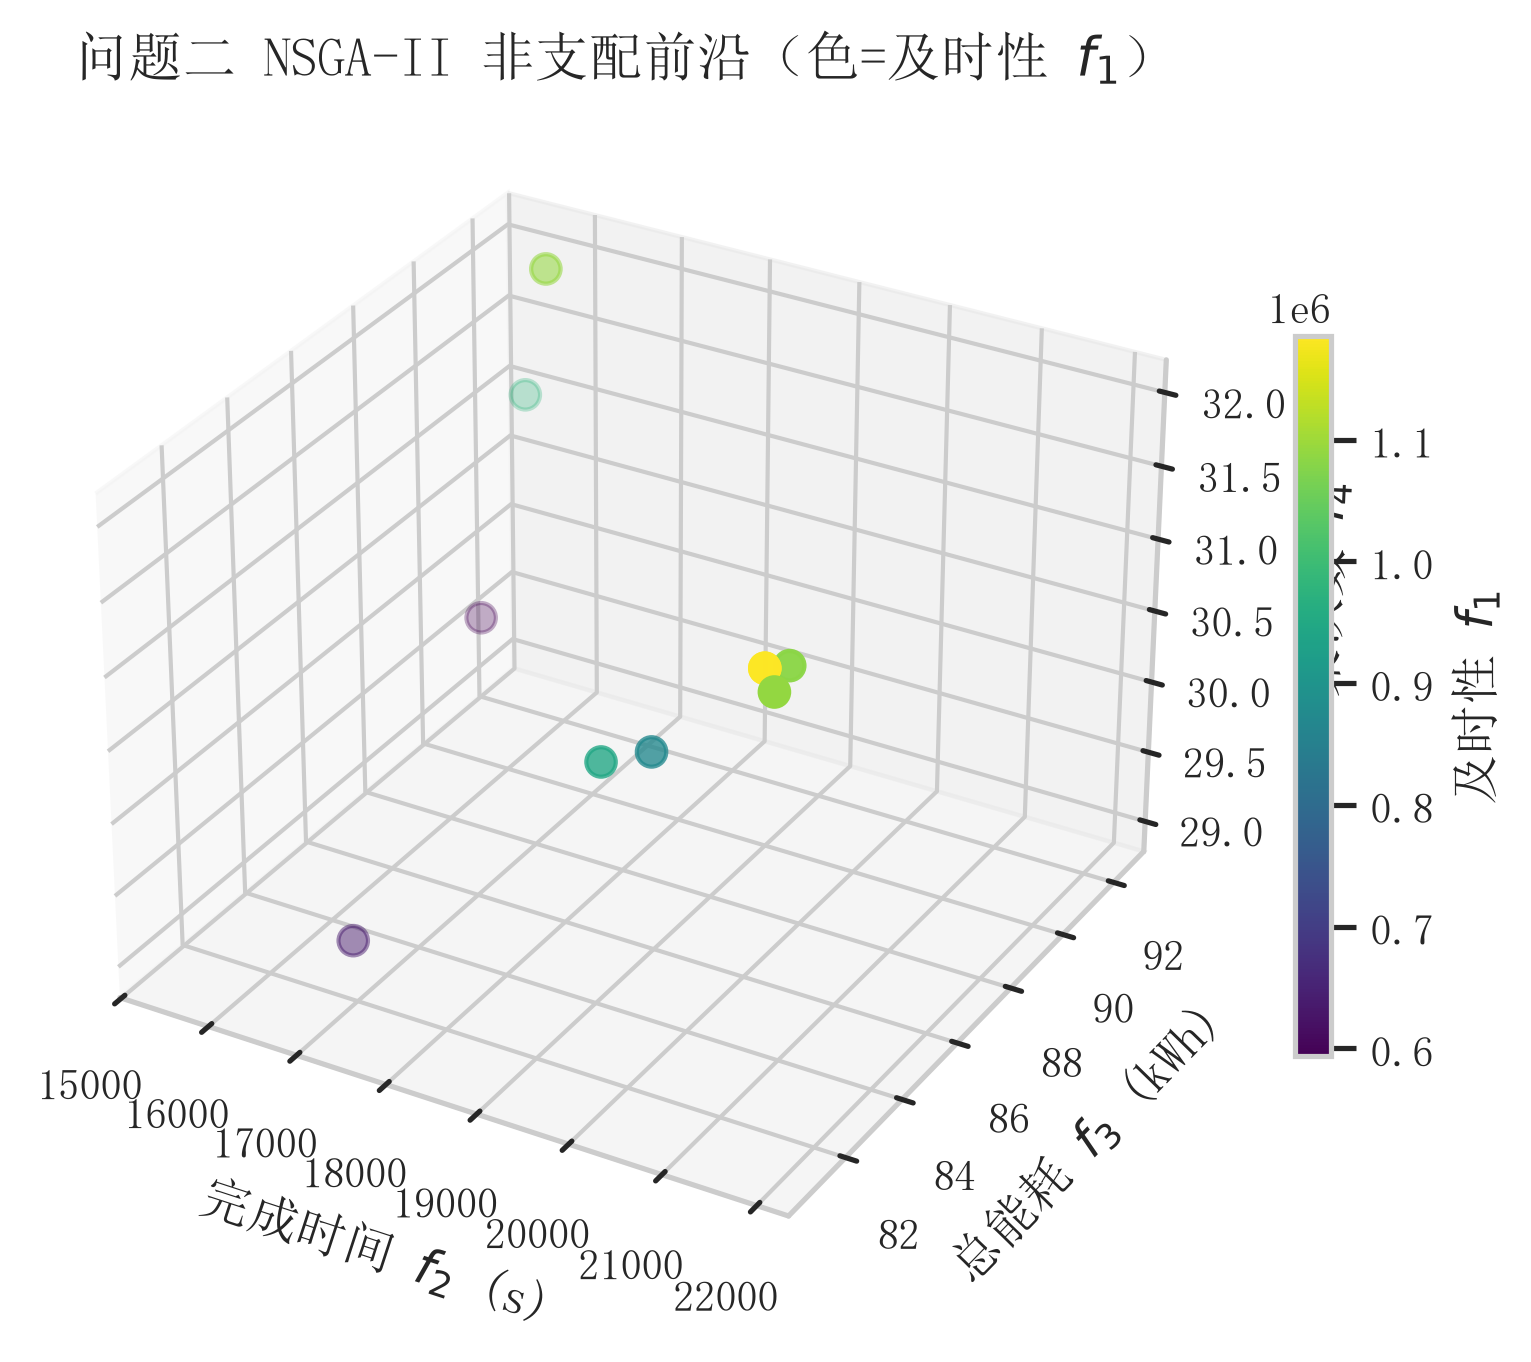
\includegraphics[width=0.48\textwidth]{figures/q2_extra_05_帕累托三维散点.png}\label{fig:q2_pareto3d}}
\caption{问题二主方案收敛过程与四目标前沿}
\label{fig:q2_conv_overview}
\end{figure}

\subsubsection{资源使用与可行性检验}

主方案的架次安排、无人机与电池分配见表~\ref{tab:q2_sorties_summary}（完整 29 架次明细见附录~\ref{app:q2_sorties}）。共享电池作为独立资源按两阶段充电周转，图~\ref{fig:q2_battery} 给出各电池的飞行/充电时长构成，可见 C 型电池飞行时长最长，与其承担的高能耗多停靠路线一致。

\begin{table}[htbp]
\centering
\caption{问题二主方案资源使用与可行性检验}
\label{tab:q2_sorties_summary}
\small
\begin{tabular}{lc}
\toprule
\textbf{检验项} & \textbf{结果} \\
\midrule
货箱覆盖 & 80/80 箱（分组编码结构性保证） \\
硬约束违反数（首批/医疗时限） & 0 \\
机队：A/B/C 型 & 4 / 2 / 2 架 \\
共享电池：A/B/C 型 & 6 / 4 / 4 组 \\
架次数（多停靠占比） & 29（7 个，24.1\%） \\
C 型架次 / B 型架次 / A 型架次 & 10 / 10 / 9 \\
总能耗 / 完成时间 & 82.777\,kWh / 16683.6\,s \\
资源占用与充电时段重叠 & 无 \\
\bottomrule
\end{tabular}
\end{table}

\begin{figure}[htbp]
\centering
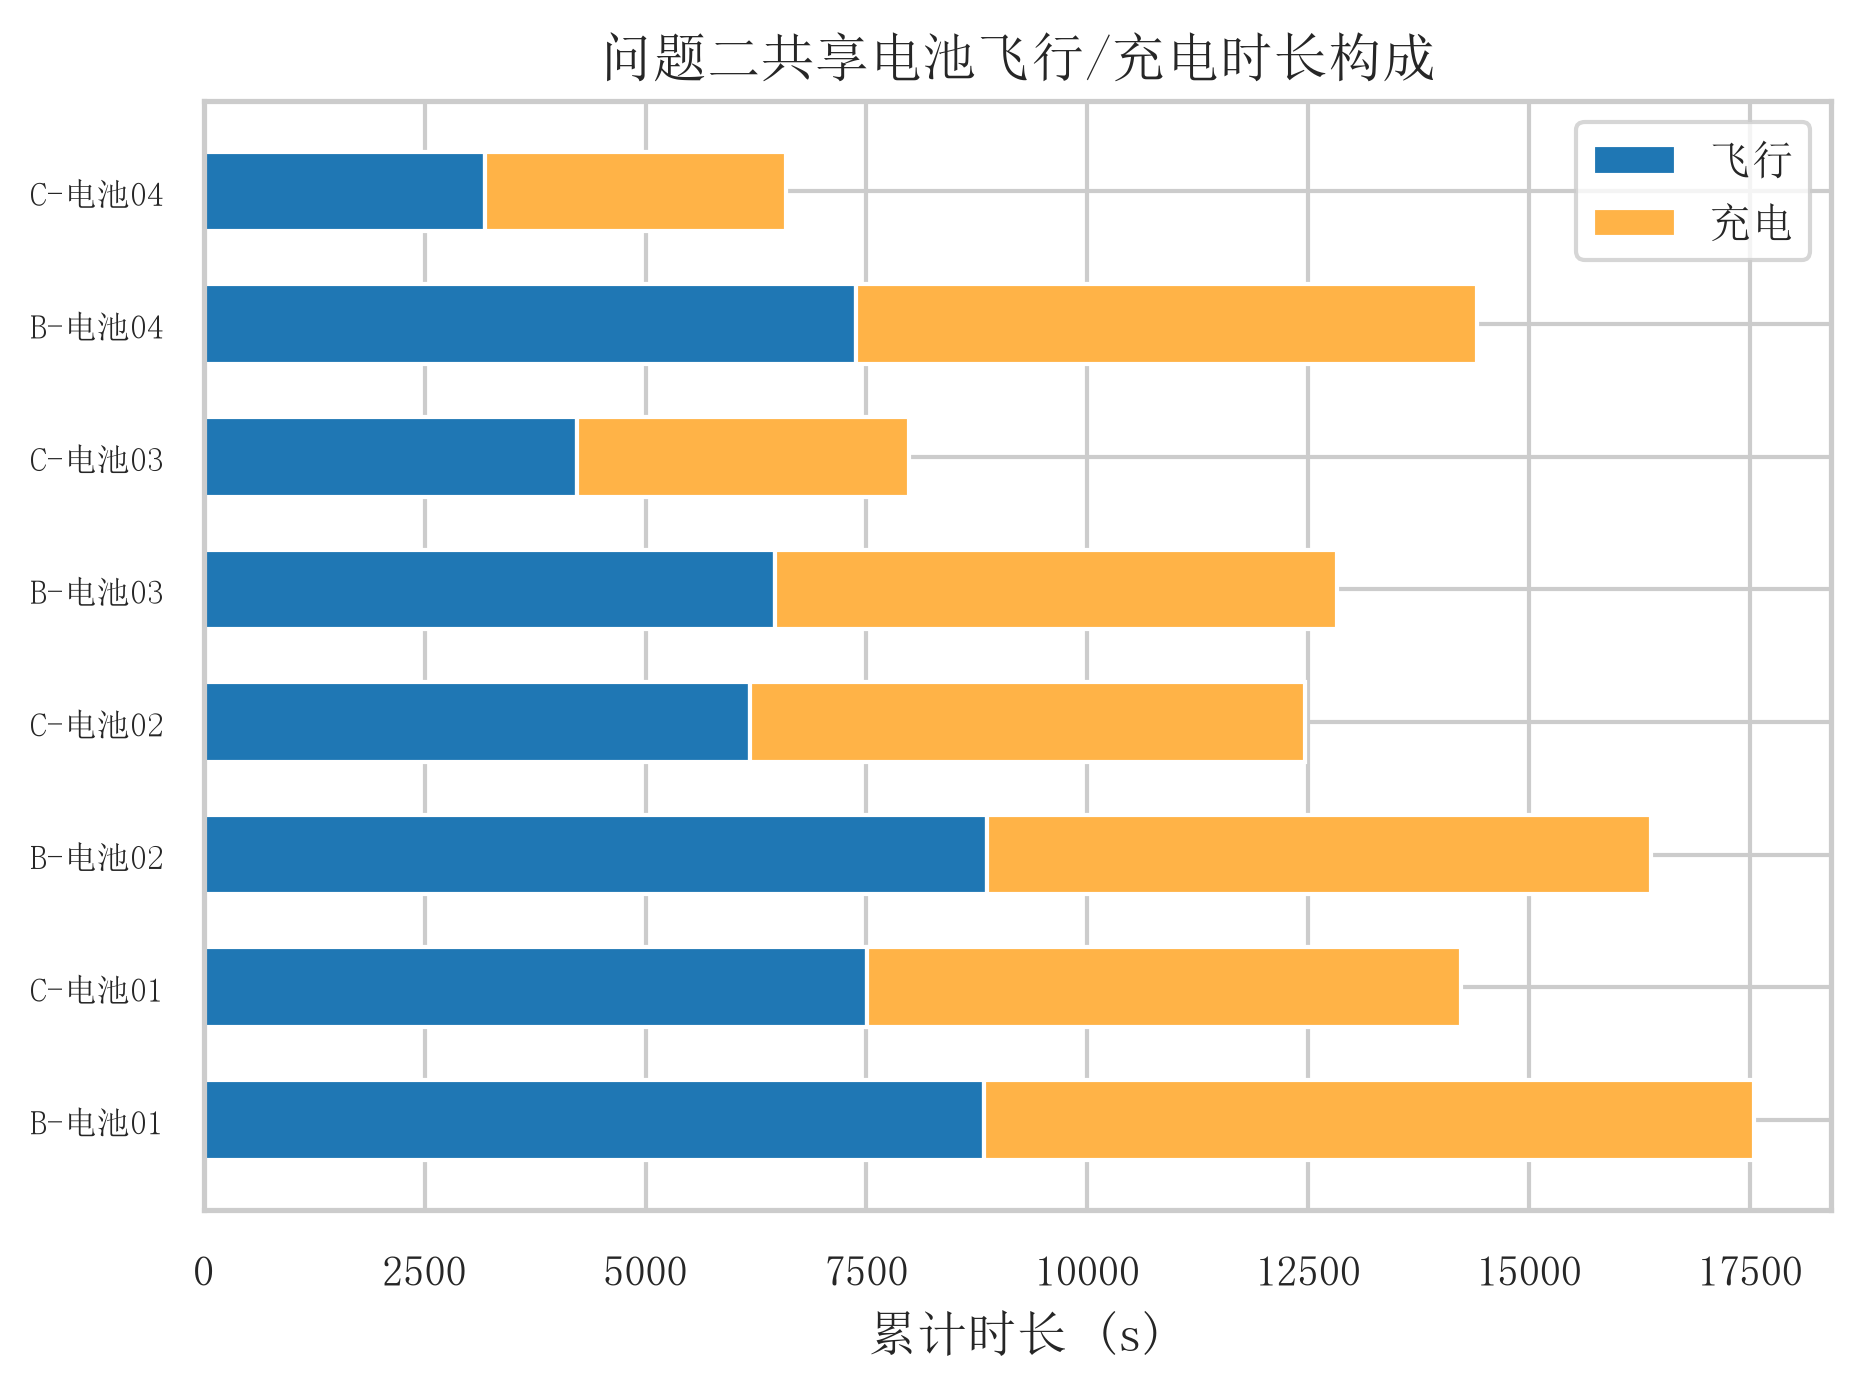
\includegraphics[width=0.72\textwidth]{figures/q2_extra_04_电池利用率.png}
\caption{问题二主方案共享电池飞行/充电时长构成}
\label{fig:q2_battery}
\end{figure}

图~\ref{fig:q2_main_gantt} 给出主方案的资源甘特图，横轴为时间、纵轴为无人机与电池资源，可见各架次在时间轴上依次排布、同一电池的飞行与充电区间互不重叠，且 C 型机身的连续任务使该机队成为 makespan 的决定性瓶颈，与表~\ref{tab:q2_sorties_summary} 的 C 型架次统计一致。

\begin{figure}[htbp]
\centering
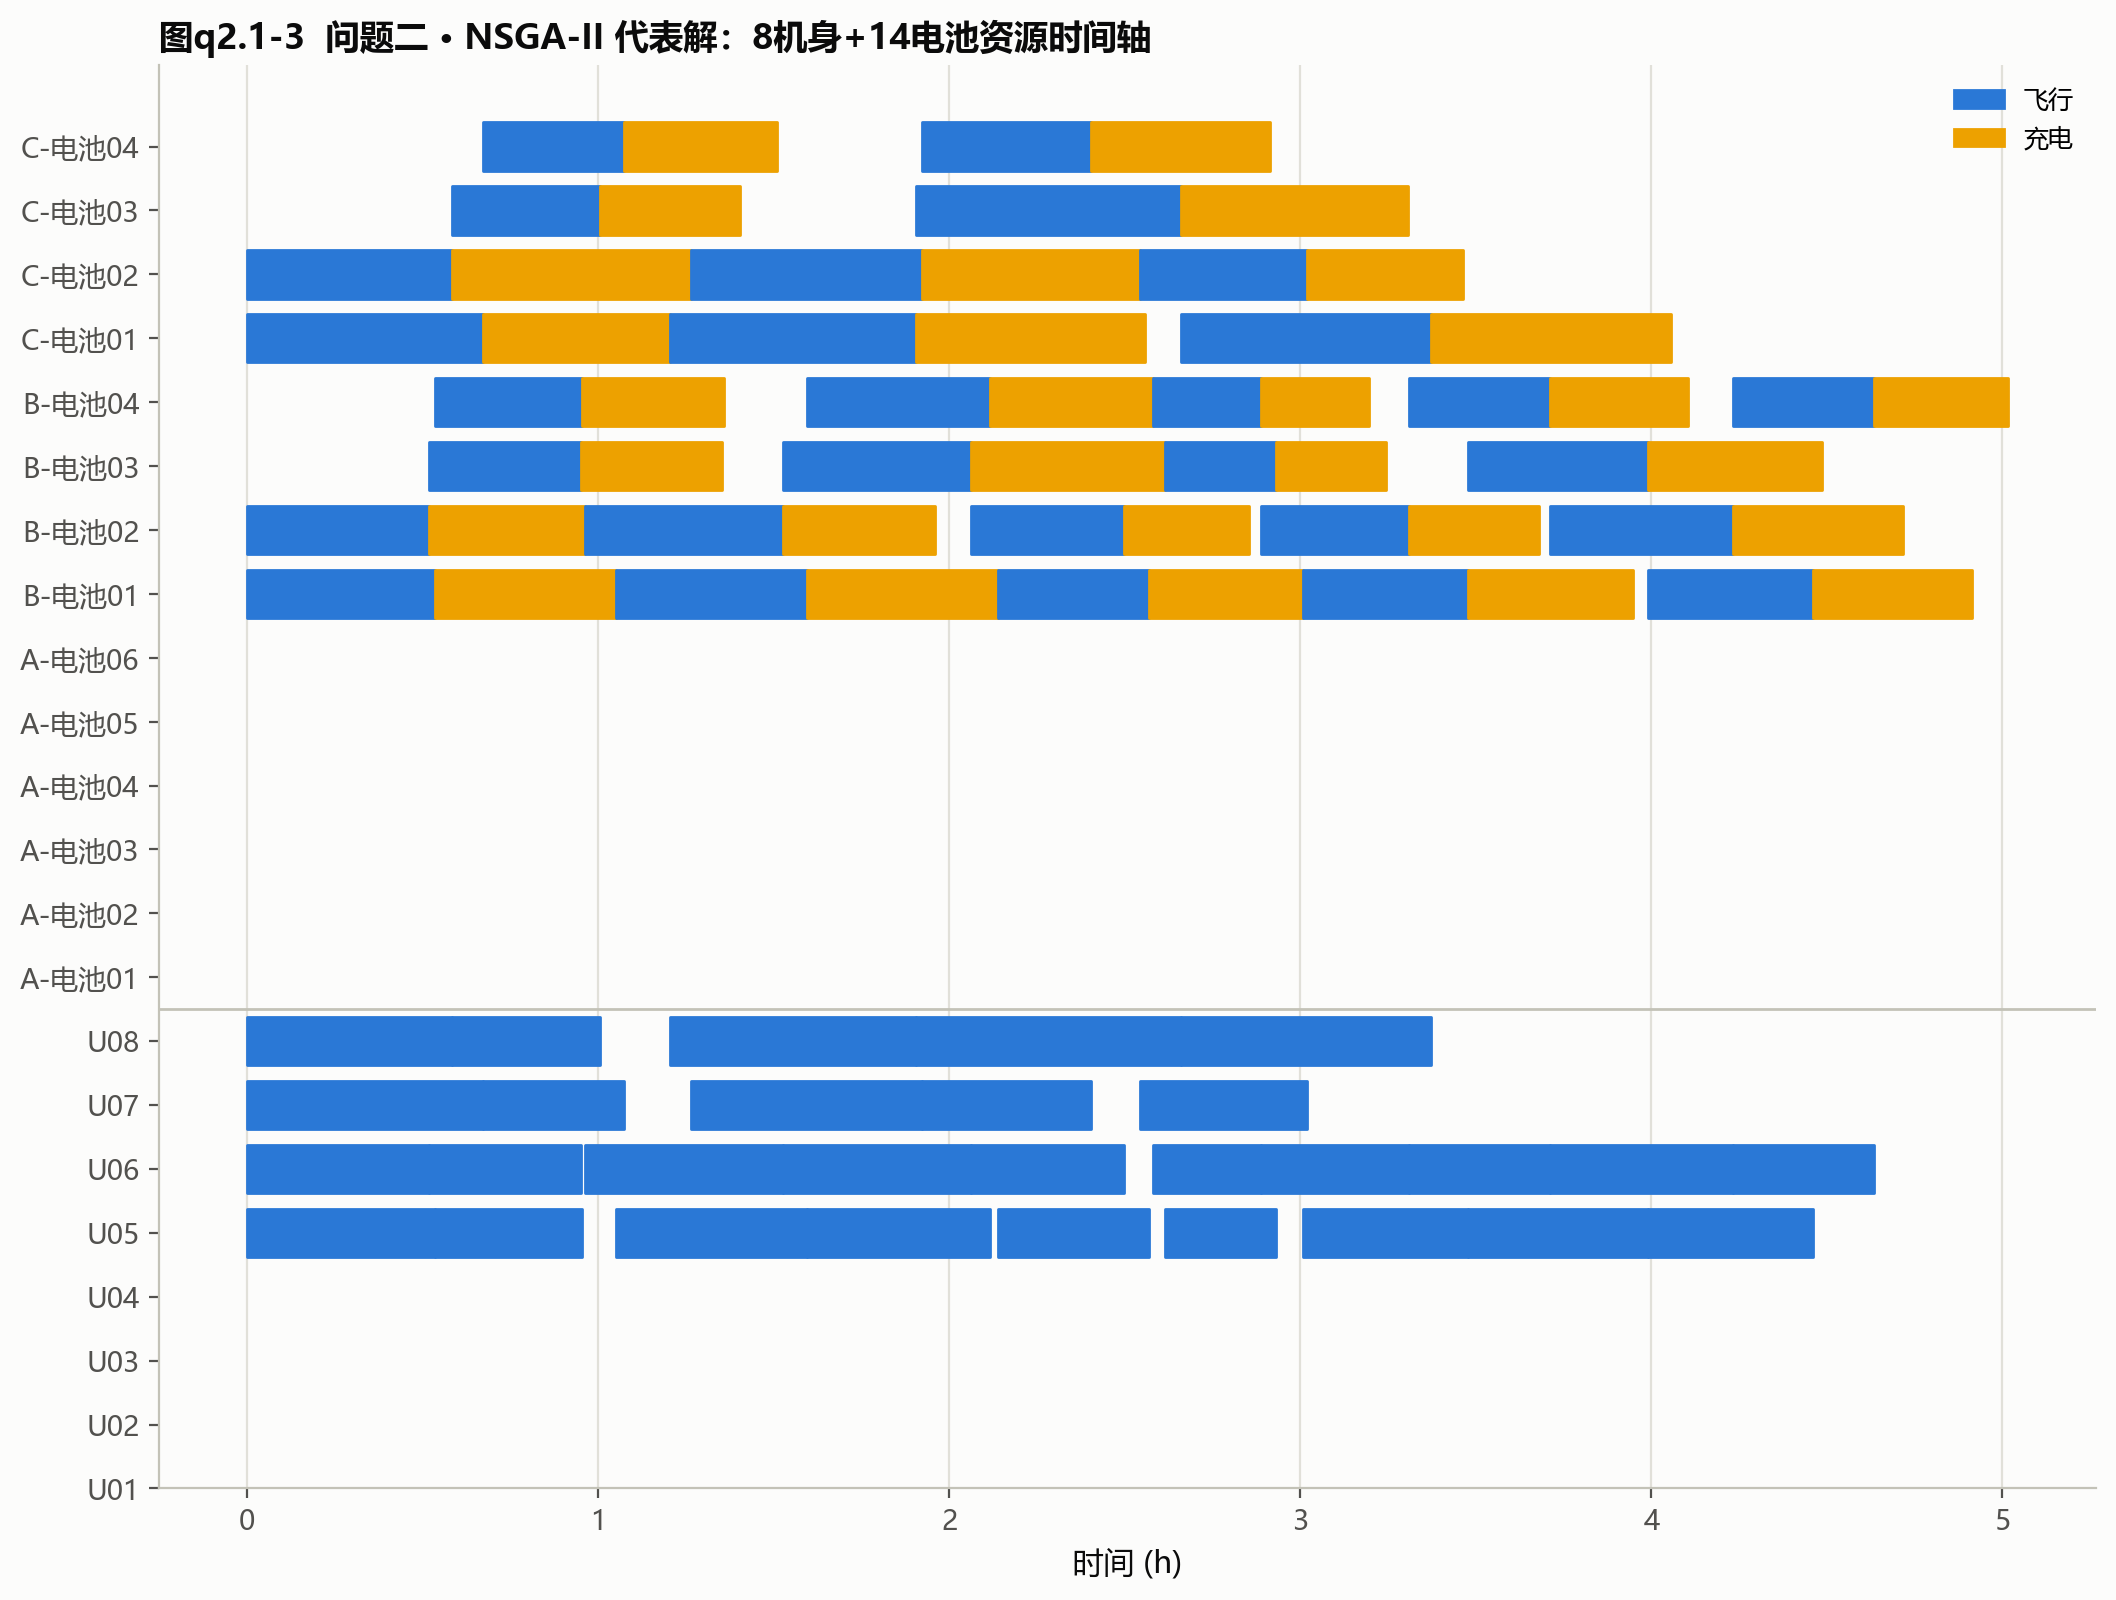
\includegraphics[width=0.9\textwidth]{figures/q2_1_03_资源甘特图.png}
\caption{问题二主方案（NSGA-II）资源甘特图}
\label{fig:q2_main_gantt}
\end{figure}

\subsection{对比方法：贪心多站合并 + 派单规则扫描}

对比方法采用构造式方法（对应代码 \texttt{q2\_2.py}），分三步，用于与主方案的严格可行解做"少架次节能"对照。

\textbf{步骤 1（基线构造）}：以问题一单站集合划分（均衡权重）得到 18 条单站路线作为起点，覆盖校验 80/80 箱通过，基线 $N_0=18$、$E_0=59.072$\,kWh、$T_0=32801.7$\,s。

\textbf{步骤 2（贪心多站合并）}：按"合并后能耗节省"对两两/三合一合并排序，全局最大优先合并，判据为合并能耗低于两站单独往返能耗之和。经 2 轮合并后，架次数由 18 降至 16（其中多停靠架次 2 个，占 12.5\%），总能耗由 59.072 降至 58.179\,kWh（节省 1.5\%），合并后箱子覆盖仍为 80/80。

\textbf{步骤 3（派单规则扫描）}：在 16 条路线上用离散事件仿真做资源排程，派单采用"紧迫覆盖优先 + 打分函数"规则——先看每条候选路线的硬时限余量，余量低于安全阈值（1800\,s）的强制排前，无紧迫路线时按打分函数（均衡 / 紧迫优先 / 能耗优先三组预设）选择。三组预设结果见表~\ref{tab:q2_dispatch}。

\begin{table}[htbp]
\centering
\caption{问题二对比方法三组派单预设结果}
\label{tab:q2_dispatch}
\small
\begin{tabular}{lcccc}
\toprule
\textbf{派单预设} & $f_1$ 及时性 & $f_2$ makespan(s) & $f_3$ 能耗(kWh) & $f_4$ 架次 \\
\midrule
均衡 & 200895.0 & 10173.7 & 58.179 & 16 \\
紧迫优先 & 200895.0 & 10173.7 & 58.179 & 16 \\
能耗优先 & 200895.0 & 10173.7 & 58.179 & 16 \\
\bottomrule
\end{tabular}
\end{table}

图~\ref{fig:q2_route} 给出对比方法的路线结构图与资源甘特图。由图可见，16 条路线均含硬时限箱（首批保障/医疗物资），"紧迫覆盖优先"规则在几乎每个派单节点都被触发，导致三组预设完全打平——这是"路线数少、每条路线普遍带硬约束箱"这一构造特点的真实结果。甘特图显示 C 型机身（仅 2 架）成为瓶颈，多停靠路线使 C/B 型机身排队，部分硬时限箱被连带拖延，最终产生 5 个硬时限违约。

\begin{figure}[htbp]
\centering
\subfloat[路线结构图]{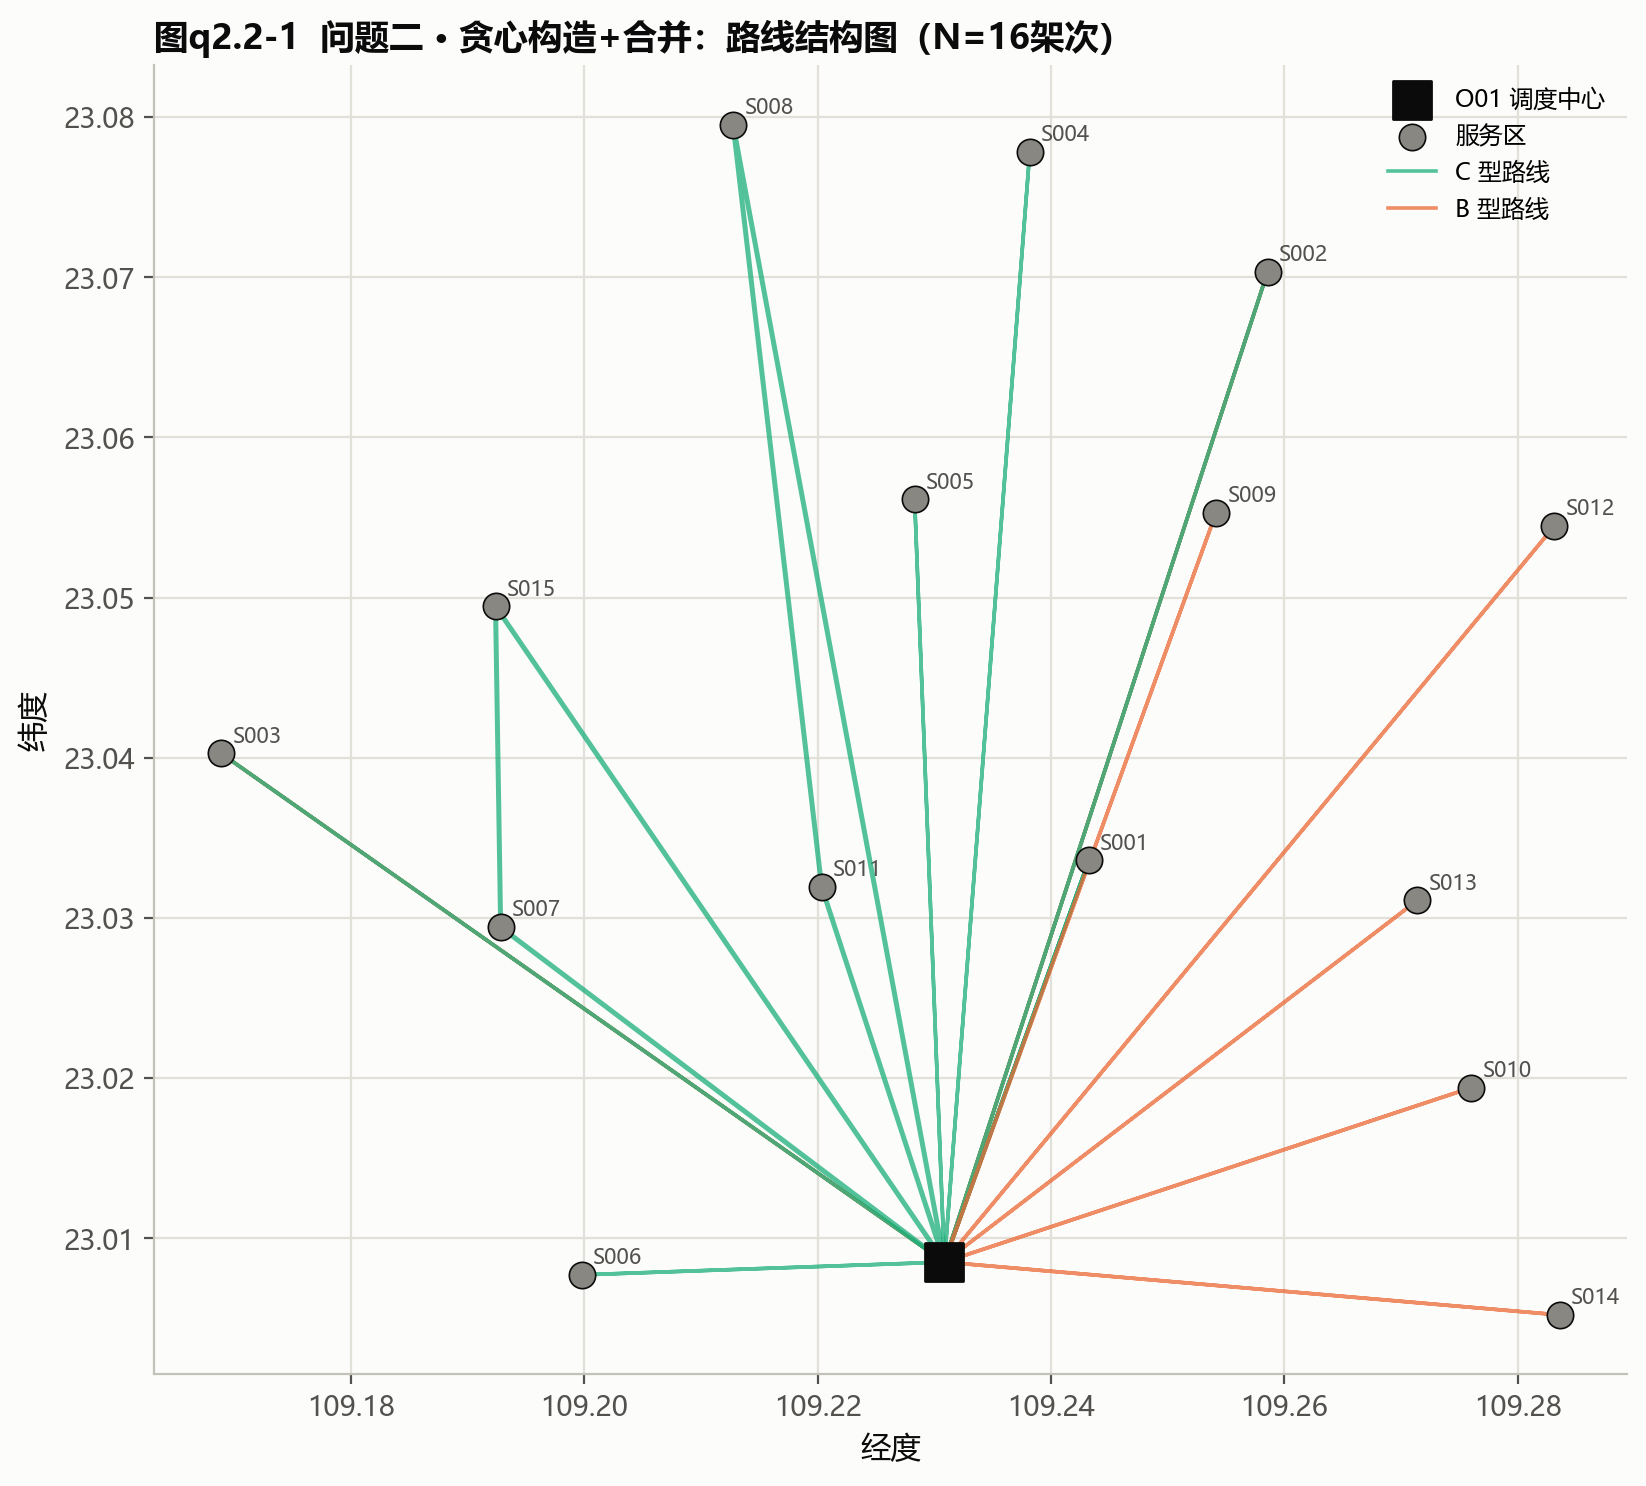
\includegraphics[width=0.48\textwidth]{figures/q2_2_01_路线结构图.png}\label{fig:q2_route}}
\hfill
\subfloat[资源甘特图]{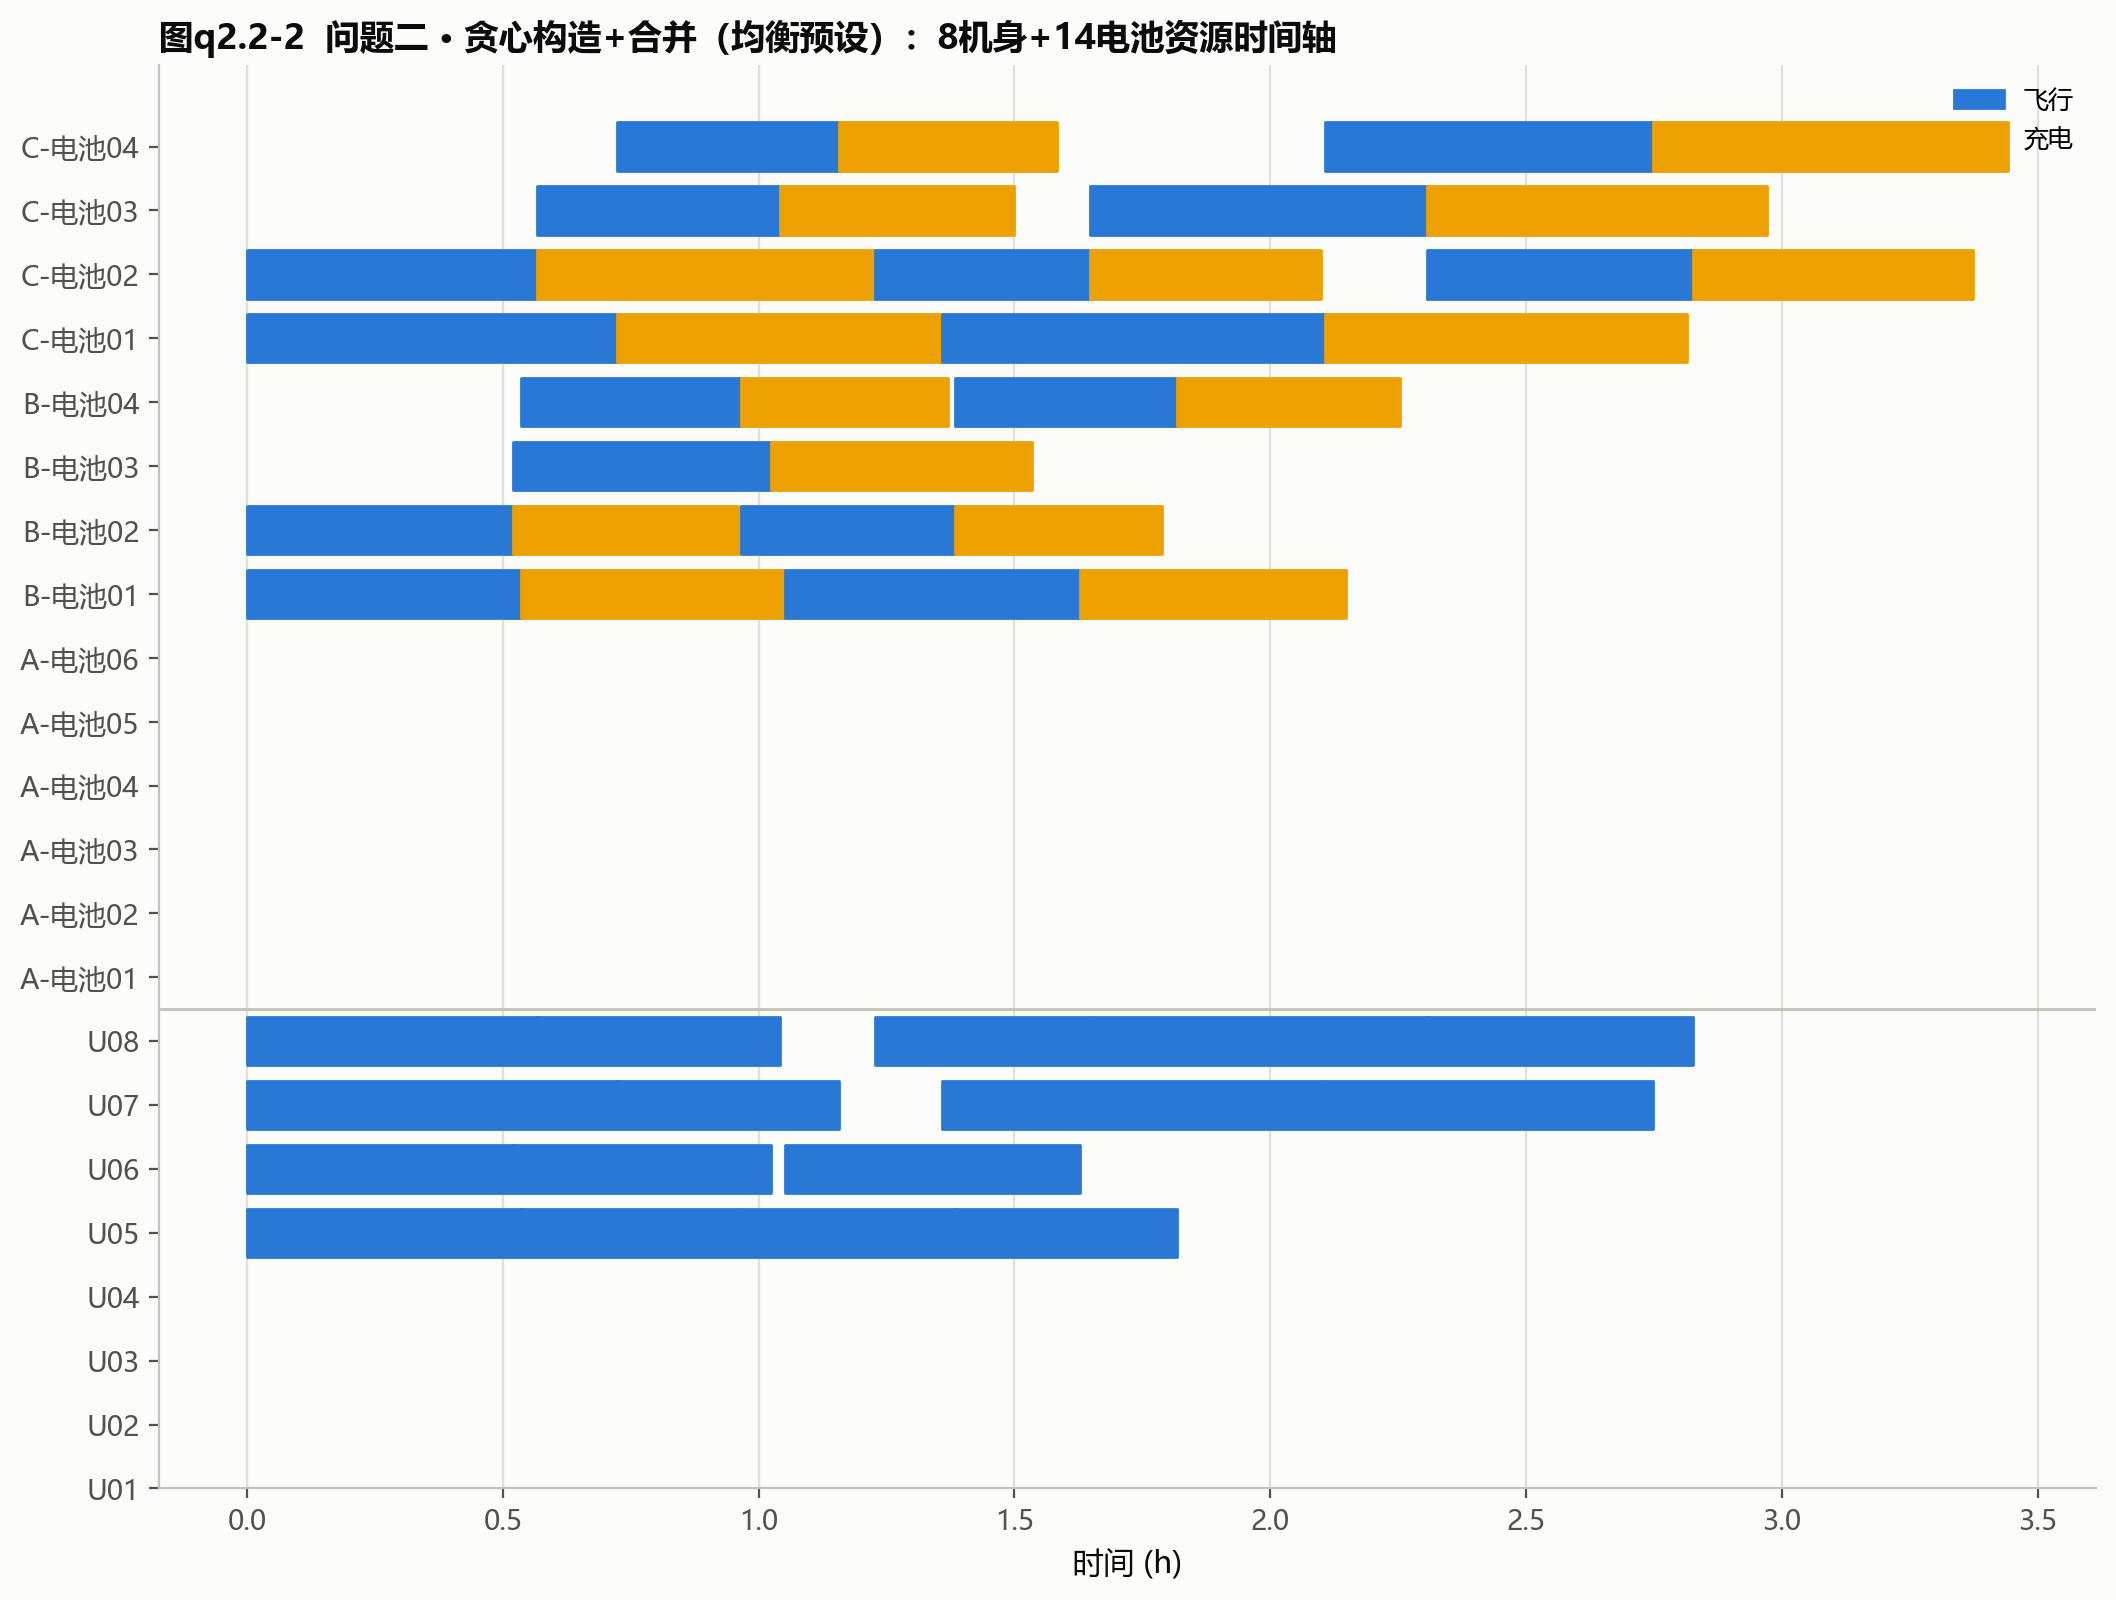
\includegraphics[width=0.48\textwidth]{figures/q2_2_02_资源甘特图.png}\label{fig:q2_gantt}}
\caption{问题二对比方法（贪心构造）路线与资源排程}
\label{fig:q2_route_overview}
\end{figure}

\subsection{模型比对与权衡分析}

两种方法的对比如表~\ref{tab:q2_compare} 与图~\ref{fig:q2_compare} 所示，揭示了两类解的典型取舍：贪心合并把更多箱子压进同一条路线，架次少、能耗低（58.179\,kWh），但路线更"重"，一旦 C/B 型机身排队，多个硬时限箱会被一起拖延，出现 5 个违反；NSGA-II 搜索了 80 代种群，主动避开拥堵分组，得到严格可行的 29 架次方案（0 违约），但能耗升至 82.777\,kWh。

\begin{table}[htbp]
\centering
\caption{问题二两种方法结果对比}
\label{tab:q2_compare}
\small
\begin{tabular}{lcccc}
\toprule
\textbf{方案} & \textbf{架次数} & \textbf{能耗(kWh)} & \textbf{makespan(s)} & \textbf{硬违约} \\
\midrule
\textbf{NSGA-II 全局优化（主方案）} & \textbf{29} & \textbf{82.777} & \textbf{16683.6} & \textbf{0} \\
贪心合并 + 派单扫描（对比） & 16 & 58.179 & 10173.7 & 5 \\
\bottomrule
\end{tabular}
\end{table}

\begin{figure}[htbp]
\centering
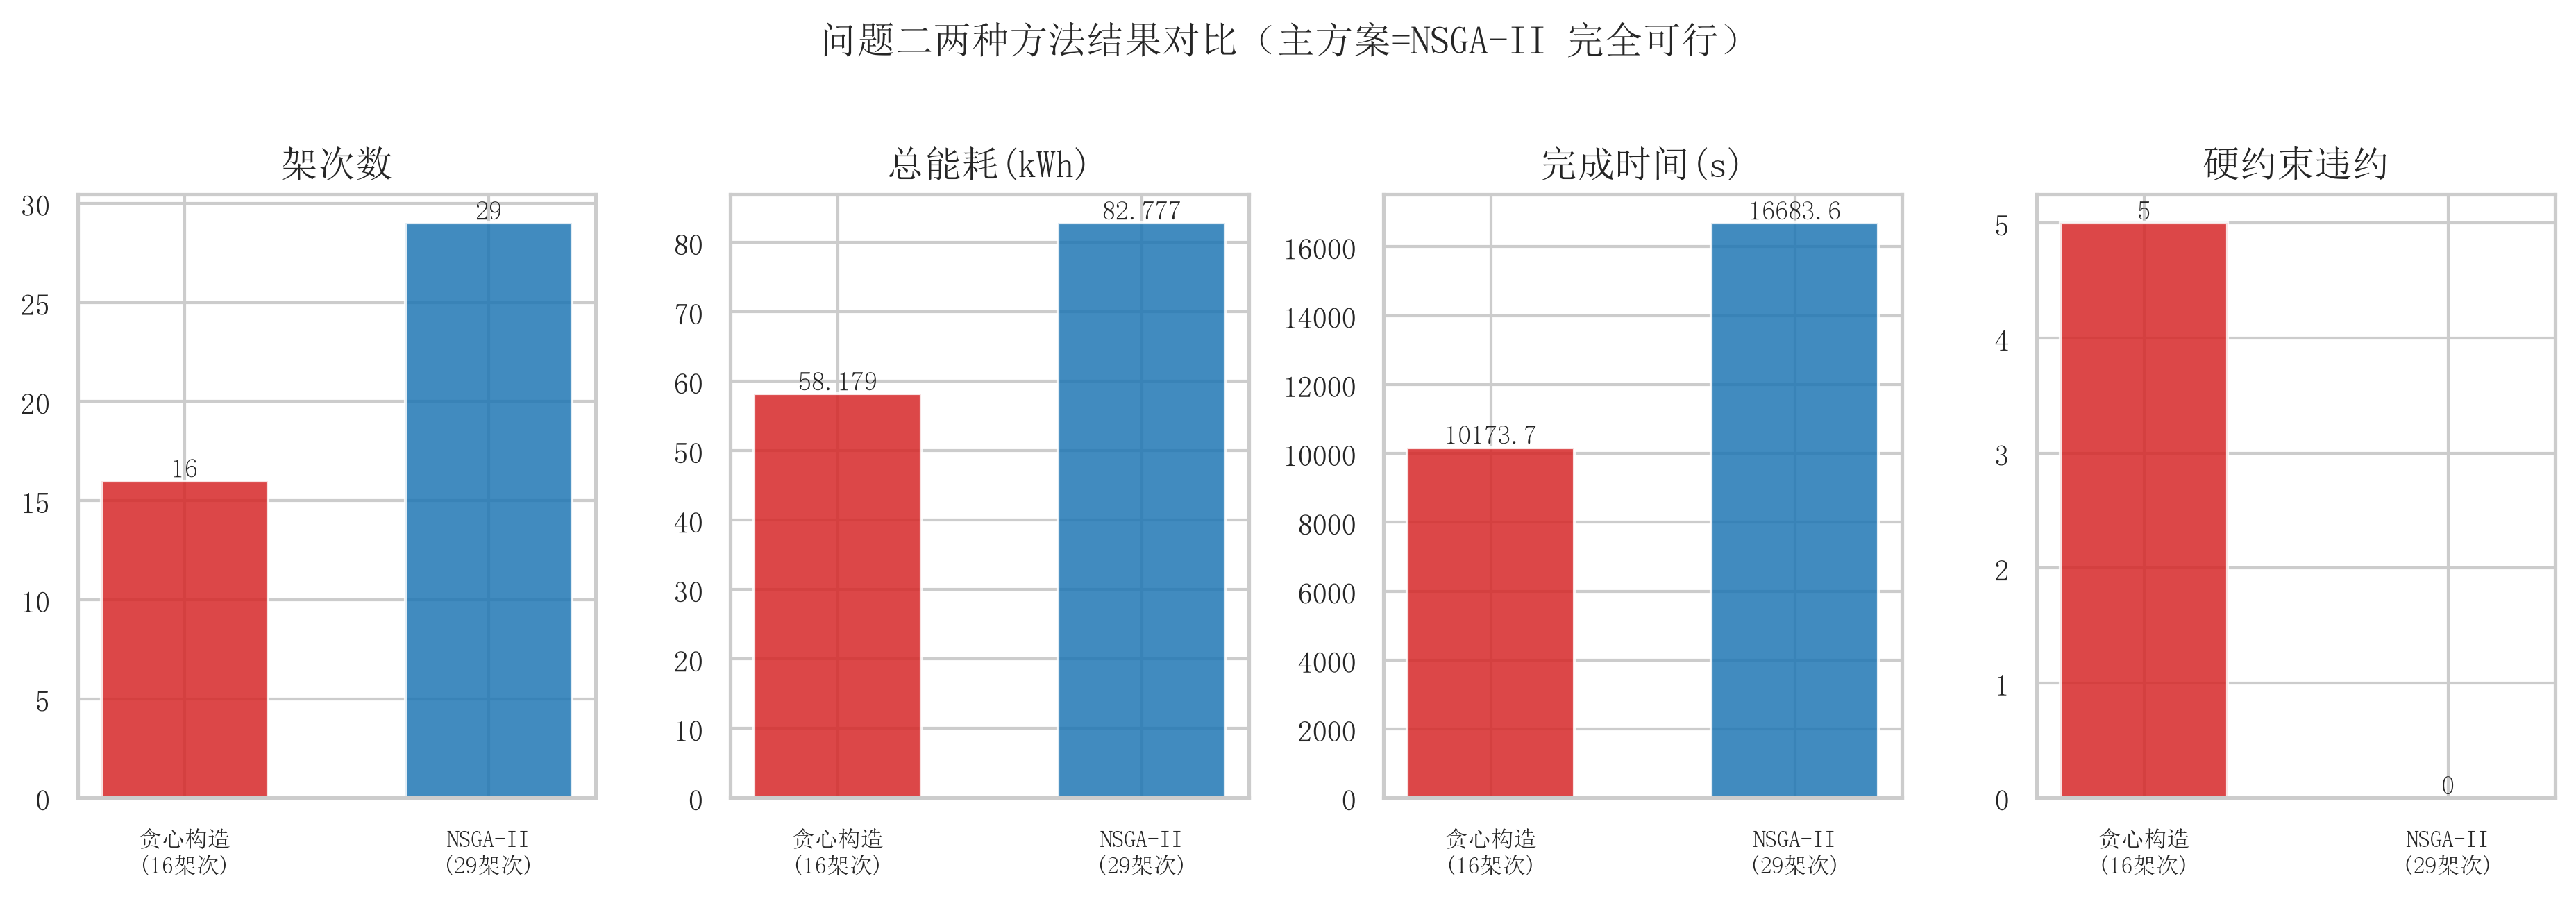
\includegraphics[width=0.95\textwidth]{figures/q2_extra_03_方法对比柱状图.png}
\caption{问题二两种方法四维指标对比}
\label{fig:q2_compare}
\end{figure}

这一权衡说明：在资源受限下，"架次更少、能耗更省"与"硬时限严格可行"并不总是兼容。对比方法（16 架次）面向"以最小能耗尽快完成大部分交付"的实用目标，其 5 个违约集中在因机身排队而被连带拖延的硬时限箱；主方案（29 架次）以更高架次与能耗换取零违约。综合"结果正确、满足全部硬约束"的求解要求，本文以 NSGA-II 严格可行解（29 架次、0 违约）为问题二主方案，其硬约束可行性也是问题三（叠加通信中继后违约进一步上升）的可解释基准。

完整的主方案运输路线明细、架次安排与逐箱送达时刻分别见附录~\ref{app:q2_routes}、\ref{app:q2_sorties}、\ref{app:q2_boxes}。
